\documentclass[twoside]{book}

% Packages required by doxygen
\usepackage{fixltx2e}
\usepackage{calc}
\usepackage{doxygen}
\usepackage[export]{adjustbox} % also loads graphicx
\usepackage{graphicx}
\usepackage[utf8]{inputenc}
\usepackage{makeidx}
\usepackage{multicol}
\usepackage{multirow}
\PassOptionsToPackage{warn}{textcomp}
\usepackage{textcomp}
\usepackage[nointegrals]{wasysym}
\usepackage[table]{xcolor}

% Font selection
\usepackage[T1]{fontenc}
\usepackage[scaled=.90]{helvet}
\usepackage{courier}
\usepackage{amssymb}
\usepackage{sectsty}
\renewcommand{\familydefault}{\sfdefault}
\allsectionsfont{%
  \fontseries{bc}\selectfont%
  \color{darkgray}%
}
\renewcommand{\DoxyLabelFont}{%
  \fontseries{bc}\selectfont%
  \color{darkgray}%
}
\newcommand{\+}{\discretionary{\mbox{\scriptsize$\hookleftarrow$}}{}{}}

% Page & text layout
\usepackage{geometry}
\geometry{%
  a4paper,%
  top=2.5cm,%
  bottom=2.5cm,%
  left=2.5cm,%
  right=2.5cm%
}
\tolerance=750
\hfuzz=15pt
\hbadness=750
\setlength{\emergencystretch}{15pt}
\setlength{\parindent}{0cm}
\setlength{\parskip}{3ex plus 2ex minus 2ex}
\makeatletter
\renewcommand{\paragraph}{%
  \@startsection{paragraph}{4}{0ex}{-1.0ex}{1.0ex}{%
    \normalfont\normalsize\bfseries\SS@parafont%
  }%
}
\renewcommand{\subparagraph}{%
  \@startsection{subparagraph}{5}{0ex}{-1.0ex}{1.0ex}{%
    \normalfont\normalsize\bfseries\SS@subparafont%
  }%
}
\makeatother

% Headers & footers
\usepackage{fancyhdr}
\pagestyle{fancyplain}
\fancyhead[LE]{\fancyplain{}{\bfseries\thepage}}
\fancyhead[CE]{\fancyplain{}{}}
\fancyhead[RE]{\fancyplain{}{\bfseries\leftmark}}
\fancyhead[LO]{\fancyplain{}{\bfseries\rightmark}}
\fancyhead[CO]{\fancyplain{}{}}
\fancyhead[RO]{\fancyplain{}{\bfseries\thepage}}
\fancyfoot[LE]{\fancyplain{}{}}
\fancyfoot[CE]{\fancyplain{}{}}
\fancyfoot[RE]{\fancyplain{}{\bfseries\scriptsize Generated by Doxygen }}
\fancyfoot[LO]{\fancyplain{}{\bfseries\scriptsize Generated by Doxygen }}
\fancyfoot[CO]{\fancyplain{}{}}
\fancyfoot[RO]{\fancyplain{}{}}
\renewcommand{\footrulewidth}{0.4pt}
\renewcommand{\chaptermark}[1]{%
  \markboth{#1}{}%
}
\renewcommand{\sectionmark}[1]{%
  \markright{\thesection\ #1}%
}

% Indices & bibliography
\usepackage{natbib}
\usepackage[titles]{tocloft}
\setcounter{tocdepth}{3}
\setcounter{secnumdepth}{5}
\makeindex

% Hyperlinks (required, but should be loaded last)
\usepackage{ifpdf}
\ifpdf
  \usepackage[pdftex,pagebackref=true]{hyperref}
\else
  \usepackage[ps2pdf,pagebackref=true]{hyperref}
\fi
\hypersetup{%
  colorlinks=true,%
  linkcolor=blue,%
  citecolor=blue,%
  unicode%
}

% Custom commands
\newcommand{\clearemptydoublepage}{%
  \newpage{\pagestyle{empty}\cleardoublepage}%
}

\usepackage{caption}
\captionsetup{labelsep=space,justification=centering,font={bf},singlelinecheck=off,skip=4pt,position=top}

%===== C O N T E N T S =====

\begin{document}

% Titlepage & ToC
\hypersetup{pageanchor=false,
             bookmarksnumbered=true,
             pdfencoding=unicode
            }
\pagenumbering{alph}
\begin{titlepage}
\vspace*{7cm}
\begin{center}%
{\Large Stock\+Market \\
{\large C++ Console Application\\}
\vspace*{1cm}
{\large Developed by André Cruz, Edgar Carneiro and João Conde}\\}
\end{center}
\end{titlepage}
\clearemptydoublepage
\pagenumbering{roman}
\tableofcontents
\clearemptydoublepage
\pagenumbering{arabic}
\hypersetup{pageanchor=true}

%--- Begin generated contents ---
\chapter{Hierarchical Index}
\section{Class Hierarchy}
This inheritance list is sorted roughly, but not completely, alphabetically\+:\begin{DoxyCompactList}
\item \contentsline{section}{Client}{\pageref{class_client}}{}
\item \contentsline{section}{Company}{\pageref{class_company}}{}
\item \contentsline{section}{Date}{\pageref{class_date}}{}
\item \contentsline{section}{Client\+:\+:Invalid\+N\+IF}{\pageref{class_client_1_1_invalid_n_i_f}}{}
\item \contentsline{section}{Order\+:\+:Invalid\+Value}{\pageref{class_order_1_1_invalid_value}}{}
\item \contentsline{section}{Investor}{\pageref{class_investor}}{}
\item \contentsline{section}{investor\+Ptr\+Hash}{\pageref{structinvestor_ptr_hash}}{}
\item \contentsline{section}{Market}{\pageref{class_market}}{}
\item \contentsline{section}{Order}{\pageref{class_order}}{}
\begin{DoxyCompactList}
\item \contentsline{section}{Buy\+Order}{\pageref{class_buy_order}}{}
\item \contentsline{section}{Sell\+Order}{\pageref{class_sell_order}}{}
\end{DoxyCompactList}
\item \contentsline{section}{Transaction}{\pageref{class_transaction}}{}
\end{DoxyCompactList}

\chapter{Class Index}
\section{Class List}
Here are the classes, structs, unions and interfaces with brief descriptions\+:\begin{DoxyCompactList}
\item\contentsline{section}{\hyperlink{class_buy_order}{Buy\+Order} }{\pageref{class_buy_order}}{}
\item\contentsline{section}{\hyperlink{class_client}{Client} }{\pageref{class_client}}{}
\item\contentsline{section}{\hyperlink{class_company}{Company} }{\pageref{class_company}}{}
\item\contentsline{section}{\hyperlink{class_date}{Date} }{\pageref{class_date}}{}
\item\contentsline{section}{\hyperlink{class_client_1_1_invalid_n_i_f}{Client\+::\+Invalid\+N\+IF} }{\pageref{class_client_1_1_invalid_n_i_f}}{}
\item\contentsline{section}{\hyperlink{class_order_1_1_invalid_value}{Order\+::\+Invalid\+Value} }{\pageref{class_order_1_1_invalid_value}}{}
\item\contentsline{section}{\hyperlink{class_investor}{Investor} }{\pageref{class_investor}}{}
\item\contentsline{section}{\hyperlink{structinvestor_ptr_hash}{investor\+Ptr\+Hash} }{\pageref{structinvestor_ptr_hash}}{}
\item\contentsline{section}{\hyperlink{class_market}{Market} }{\pageref{class_market}}{}
\item\contentsline{section}{\hyperlink{class_order}{Order} }{\pageref{class_order}}{}
\item\contentsline{section}{\hyperlink{class_sell_order}{Sell\+Order} }{\pageref{class_sell_order}}{}
\item\contentsline{section}{\hyperlink{class_transaction}{Transaction} }{\pageref{class_transaction}}{}
\end{DoxyCompactList}

\chapter{Class Documentation}
\hypertarget{class_buy_order}{}\section{Buy\+Order Class Reference}
\label{class_buy_order}\index{Buy\+Order@{Buy\+Order}}


{\ttfamily \#include $<$Order.\+h$>$}

Inheritance diagram for Buy\+Order\+:\begin{figure}[H]
\begin{center}
\leavevmode
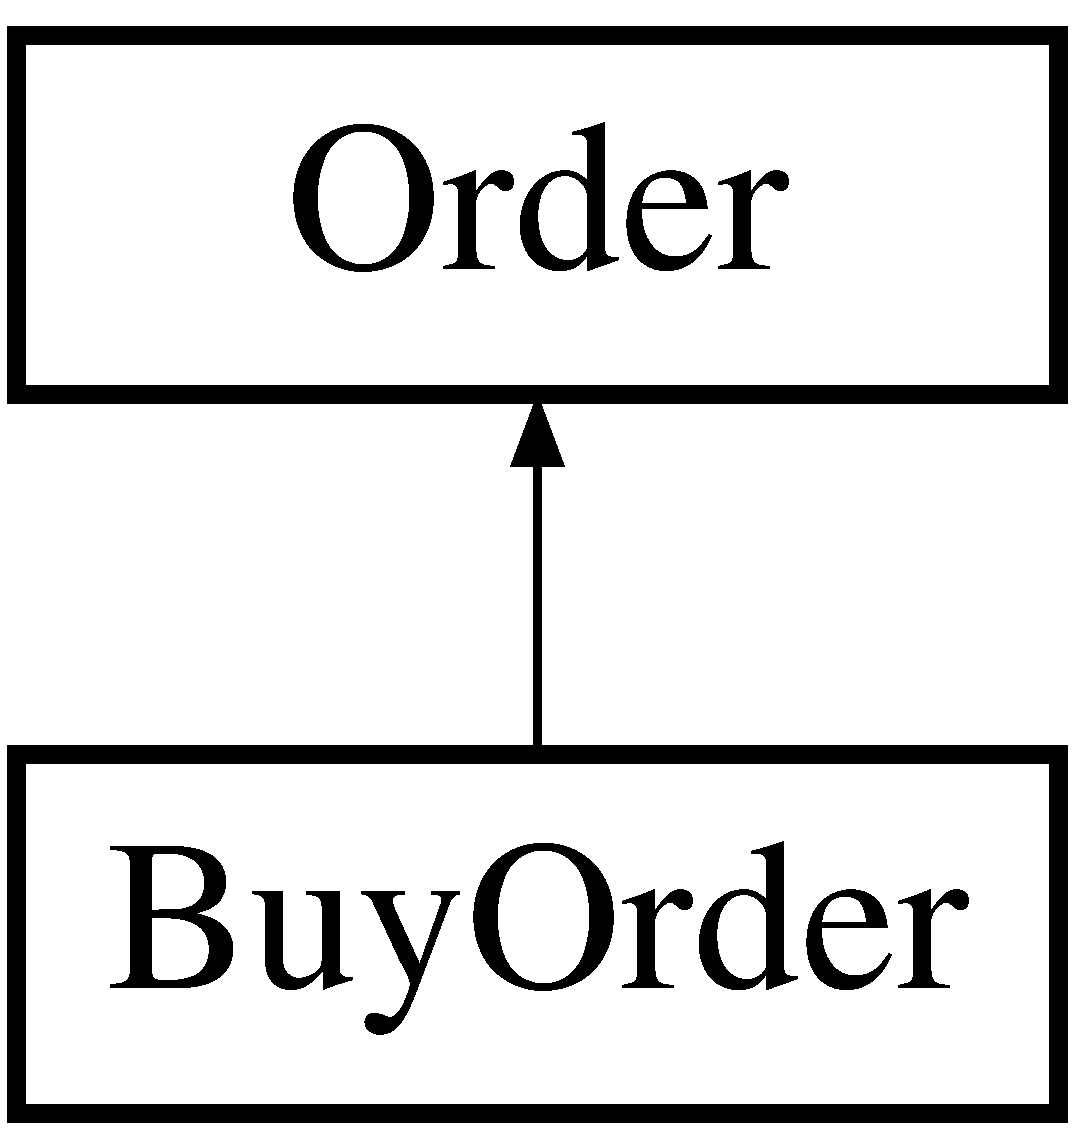
\includegraphics[height=2.000000cm]{class_buy_order}
\end{center}
\end{figure}
\subsection*{Public Member Functions}
\begin{DoxyCompactItemize}
\item 
\hyperlink{class_buy_order_acbf093767d9d108b9448f2eefb5f58cd}{Buy\+Order} (ifstream \&in)
\begin{DoxyCompactList}\small\item\em /// \end{DoxyCompactList}\item 
\hyperlink{class_buy_order_a1fcd1c4a28acdf04bfdf99c5b16b4e7d}{Buy\+Order} (string \hyperlink{class_order_aafb6dfab2a1c253eefd78840b27dcd2e}{stock}, double val, unsigned \hyperlink{class_order_ab02e2baeb8c57217a20c9124df3ba11d}{quantity}, nif\+\_\+t \hyperlink{class_buy_order_a5914aebb1dd8bb32d1b7481235d833fc}{buyer\+N\+IF})
\item 
nif\+\_\+t \hyperlink{class_buy_order_ab79597b9bf0656216b2283bfa3a650e0}{get\+Client\+N\+IF} () const
\item 
\hyperlink{class_transaction}{Transaction} $\ast$ \hyperlink{class_buy_order_a45641eed13ea191fff675745a618b9f5}{operator()} (\hyperlink{class_order}{Order} $\ast$o)
\item 
void \hyperlink{class_buy_order_aa4f087d0dbc1f6e8937c0b3679fc2f7b}{save\+Changes} (ofstream \&out) const
\end{DoxyCompactItemize}
\subsection*{Private Attributes}
\begin{DoxyCompactItemize}
\item 
\mbox{\Hypertarget{class_buy_order_ac67ae4ec42300c879e4bfd2e2cd2adb2}\label{class_buy_order_ac67ae4ec42300c879e4bfd2e2cd2adb2}} 
friend {\bfseries Sell\+Order}
\item 
nif\+\_\+t \hyperlink{class_buy_order_a5914aebb1dd8bb32d1b7481235d833fc}{buyer\+N\+IF}
\end{DoxyCompactItemize}
\subsection*{Additional Inherited Members}


\subsection{Detailed Description}
Class used to represent a buy order. Derives from \hyperlink{class_order}{Order}. 

\subsection{Constructor \& Destructor Documentation}
\mbox{\Hypertarget{class_buy_order_acbf093767d9d108b9448f2eefb5f58cd}\label{class_buy_order_acbf093767d9d108b9448f2eefb5f58cd}} 
\index{Buy\+Order@{Buy\+Order}!Buy\+Order@{Buy\+Order}}
\index{Buy\+Order@{Buy\+Order}!Buy\+Order@{Buy\+Order}}
\subsubsection{\texorpdfstring{Buy\+Order()}{BuyOrder()}\hspace{0.1cm}{\footnotesize\ttfamily [1/2]}}
{\footnotesize\ttfamily Buy\+Order\+::\+Buy\+Order (\begin{DoxyParamCaption}\item[{ifstream \&}]{in }\end{DoxyParamCaption})}



/// 

A constructor. The construtor creates a \hyperlink{class_buy_order}{Buy\+Order} object, reading the data from the input stream passed as argument. 
\begin{DoxyParams}{Parameters}
{\em in} & The input stream to read from in order to build the \hyperlink{class_buy_order}{Buy\+Order} object. \\
\hline
\end{DoxyParams}
\mbox{\Hypertarget{class_buy_order_a1fcd1c4a28acdf04bfdf99c5b16b4e7d}\label{class_buy_order_a1fcd1c4a28acdf04bfdf99c5b16b4e7d}} 
\index{Buy\+Order@{Buy\+Order}!Buy\+Order@{Buy\+Order}}
\index{Buy\+Order@{Buy\+Order}!Buy\+Order@{Buy\+Order}}
\subsubsection{\texorpdfstring{Buy\+Order()}{BuyOrder()}\hspace{0.1cm}{\footnotesize\ttfamily [2/2]}}
{\footnotesize\ttfamily Buy\+Order\+::\+Buy\+Order (\begin{DoxyParamCaption}\item[{string}]{stock,  }\item[{double}]{val,  }\item[{unsigned}]{quantity,  }\item[{nif\+\_\+t}]{buyer\+N\+IF }\end{DoxyParamCaption})}

A constructor. The construtor creates a \hyperlink{class_buy_order}{Buy\+Order} object using the data passed as arguments. 
\begin{DoxyParams}{Parameters}
{\em stock} & A string with the stock name. \\
\hline
{\em val} & A double with the value per stock. \\
\hline
{\em quantity} & An unsigned with the stock quantity. \\
\hline
{\em buyer\+N\+IF} & The buyer\textquotesingle{}s N\+IF. \\
\hline
\end{DoxyParams}


\subsection{Member Function Documentation}
\mbox{\Hypertarget{class_buy_order_ab79597b9bf0656216b2283bfa3a650e0}\label{class_buy_order_ab79597b9bf0656216b2283bfa3a650e0}} 
\index{Buy\+Order@{Buy\+Order}!get\+Client\+N\+IF@{get\+Client\+N\+IF}}
\index{get\+Client\+N\+IF@{get\+Client\+N\+IF}!Buy\+Order@{Buy\+Order}}
\subsubsection{\texorpdfstring{get\+Client\+N\+I\+F()}{getClientNIF()}}
{\footnotesize\ttfamily nif\+\_\+t Buy\+Order\+::get\+Client\+N\+IF (\begin{DoxyParamCaption}{ }\end{DoxyParamCaption}) const\hspace{0.3cm}{\ttfamily [virtual]}}

A const member function that returns the N\+IF of the client associated with this \hyperlink{class_buy_order}{Buy\+Order}. \begin{DoxyReturn}{Returns}
The N\+IF of the Buyer associated with this \hyperlink{class_order}{Order}. 
\end{DoxyReturn}


Implements \hyperlink{class_order_a9831f386726f74ee20eea13a46282e13}{Order}.

\mbox{\Hypertarget{class_buy_order_a45641eed13ea191fff675745a618b9f5}\label{class_buy_order_a45641eed13ea191fff675745a618b9f5}} 
\index{Buy\+Order@{Buy\+Order}!operator()@{operator()}}
\index{operator()@{operator()}!Buy\+Order@{Buy\+Order}}
\subsubsection{\texorpdfstring{operator()()}{operator()()}}
{\footnotesize\ttfamily \hyperlink{class_transaction}{Transaction} $\ast$ Buy\+Order\+::operator() (\begin{DoxyParamCaption}\item[{\hyperlink{class_order}{Order} $\ast$}]{o }\end{DoxyParamCaption})\hspace{0.3cm}{\ttfamily [virtual]}}

Overload of operator() for class \hyperlink{class_order}{Order}. 
\begin{DoxyParams}{Parameters}
{\em o} & Pointer of an object \hyperlink{class_order}{Order}. \\
\hline
\end{DoxyParams}
\begin{DoxyReturn}{Returns}
A transaction type object. 
\end{DoxyReturn}


Implements \hyperlink{class_order_a85d5de18c8664085619e3a5c74d47a25}{Order}.

\mbox{\Hypertarget{class_buy_order_aa4f087d0dbc1f6e8937c0b3679fc2f7b}\label{class_buy_order_aa4f087d0dbc1f6e8937c0b3679fc2f7b}} 
\index{Buy\+Order@{Buy\+Order}!save\+Changes@{save\+Changes}}
\index{save\+Changes@{save\+Changes}!Buy\+Order@{Buy\+Order}}
\subsubsection{\texorpdfstring{save\+Changes()}{saveChanges()}}
{\footnotesize\ttfamily void Buy\+Order\+::save\+Changes (\begin{DoxyParamCaption}\item[{ofstream \&}]{out }\end{DoxyParamCaption}) const\hspace{0.3cm}{\ttfamily [virtual]}}

A const memeber function to save changes in an output stream. 
\begin{DoxyParams}{Parameters}
{\em out} & The outstream file to write to. \\
\hline
\end{DoxyParams}


Reimplemented from \hyperlink{class_order_a83989bde0a9b40cbeb0e87c965f6096e}{Order}.



\subsection{Member Data Documentation}
\mbox{\Hypertarget{class_buy_order_a5914aebb1dd8bb32d1b7481235d833fc}\label{class_buy_order_a5914aebb1dd8bb32d1b7481235d833fc}} 
\index{Buy\+Order@{Buy\+Order}!buyer\+N\+IF@{buyer\+N\+IF}}
\index{buyer\+N\+IF@{buyer\+N\+IF}!Buy\+Order@{Buy\+Order}}
\subsubsection{\texorpdfstring{buyer\+N\+IF}{buyerNIF}}
{\footnotesize\ttfamily nif\+\_\+t Buy\+Order\+::buyer\+N\+IF\hspace{0.3cm}{\ttfamily [private]}}

nif\+\_\+t buyer\+N\+IF. The N\+IF of the buyer associated with this \hyperlink{class_order}{Order}. 

The documentation for this class was generated from the following files\+:\begin{DoxyCompactItemize}
\item 
D\+:/\+Projetos\+C++/\+A\+E\+D\+Av2/\+Stock\+Market/Order.\+h\item 
D\+:/\+Projetos\+C++/\+A\+E\+D\+Av2/\+Stock\+Market/Order.\+cpp\end{DoxyCompactItemize}

\hypertarget{class_client}{}\section{Client Class Reference}
\label{class_client}\index{Client@{Client}}


{\ttfamily \#include $<$Client.\+h$>$}

\subsection*{Classes}
\begin{DoxyCompactItemize}
\item 
class \hyperlink{class_client_1_1_invalid_n_i_f}{Invalid\+N\+IF}
\end{DoxyCompactItemize}
\subsection*{Public Member Functions}
\begin{DoxyCompactItemize}
\item 
\hyperlink{class_client_ac13ad1e98c47db57ce0823dc735261cd}{Client} ()=default
\item 
\hyperlink{class_client_a978037b72169d091a54867507ecd38ed}{Client} (ifstream \&in)
\item 
\hyperlink{class_client_a756361657c5f81a798583456fb82b128}{Client} (string \hyperlink{class_client_a456e36f9972a8bf3ecdb5f0e70b3bd5d}{name}, nif\+\_\+t \hyperlink{class_client_a80e87b7c418824a3ebfafaf6f3fc8b3d}{nif})
\item 
string \hyperlink{class_client_a5c473ba52d7678744edec9e51052c947}{get\+Name} () const
\item 
nif\+\_\+t \hyperlink{class_client_a2f9bc46f381dcbd0f35929f54dabad59}{get\+N\+IF} () const
\item 
void \hyperlink{class_client_a3bd7a77458497b3b863b7c7515d76e68}{save\+Changes} (ofstream \&out) const
\end{DoxyCompactItemize}
\subsection*{Private Attributes}
\begin{DoxyCompactItemize}
\item 
string \hyperlink{class_client_a456e36f9972a8bf3ecdb5f0e70b3bd5d}{name}
\item 
nif\+\_\+t \hyperlink{class_client_a80e87b7c418824a3ebfafaf6f3fc8b3d}{nif}
\end{DoxyCompactItemize}


\subsection{Detailed Description}
A class used to represent a client. Each client object has a name and a nif (from the portuguese \char`\"{}\+Numero de Identifica��o Fiscal\char`\"{}). 

\subsection{Constructor \& Destructor Documentation}
\mbox{\Hypertarget{class_client_ac13ad1e98c47db57ce0823dc735261cd}\label{class_client_ac13ad1e98c47db57ce0823dc735261cd}} 
\index{Client@{Client}!Client@{Client}}
\index{Client@{Client}!Client@{Client}}
\subsubsection{\texorpdfstring{Client()}{Client()}\hspace{0.1cm}{\footnotesize\ttfamily [1/3]}}
{\footnotesize\ttfamily Client\+::\+Client (\begin{DoxyParamCaption}{ }\end{DoxyParamCaption})\hspace{0.3cm}{\ttfamily [default]}}

A default constructor. \mbox{\Hypertarget{class_client_a978037b72169d091a54867507ecd38ed}\label{class_client_a978037b72169d091a54867507ecd38ed}} 
\index{Client@{Client}!Client@{Client}}
\index{Client@{Client}!Client@{Client}}
\subsubsection{\texorpdfstring{Client()}{Client()}\hspace{0.1cm}{\footnotesize\ttfamily [2/3]}}
{\footnotesize\ttfamily Client\+::\+Client (\begin{DoxyParamCaption}\item[{ifstream \&}]{in }\end{DoxyParamCaption})}

A constructor. The construtor creates a \hyperlink{class_client}{Client} object, reading the data from the input stream passed as argument. 
\begin{DoxyParams}{Parameters}
{\em in} & The input stream to read from in order to build the client object. \\
\hline
\end{DoxyParams}
\mbox{\Hypertarget{class_client_a756361657c5f81a798583456fb82b128}\label{class_client_a756361657c5f81a798583456fb82b128}} 
\index{Client@{Client}!Client@{Client}}
\index{Client@{Client}!Client@{Client}}
\subsubsection{\texorpdfstring{Client()}{Client()}\hspace{0.1cm}{\footnotesize\ttfamily [3/3]}}
{\footnotesize\ttfamily Client\+::\+Client (\begin{DoxyParamCaption}\item[{string}]{name,  }\item[{nif\+\_\+t}]{nif }\end{DoxyParamCaption})}

A constructor. The construtor creates a client object with the data passed as arguments. 
\begin{DoxyParams}{Parameters}
{\em name} & The client\textquotesingle{}s name. \\
\hline
{\em nif} & The client\textquotesingle{}s N\+IF. \\
\hline
\end{DoxyParams}


\subsection{Member Function Documentation}
\mbox{\Hypertarget{class_client_a5c473ba52d7678744edec9e51052c947}\label{class_client_a5c473ba52d7678744edec9e51052c947}} 
\index{Client@{Client}!get\+Name@{get\+Name}}
\index{get\+Name@{get\+Name}!Client@{Client}}
\subsubsection{\texorpdfstring{get\+Name()}{getName()}}
{\footnotesize\ttfamily string Client\+::get\+Name (\begin{DoxyParamCaption}{ }\end{DoxyParamCaption}) const}

A const member function with no arguments to get the client\textquotesingle{}s name. \begin{DoxyReturn}{Returns}
A string, the client\textquotesingle{}s name. 
\end{DoxyReturn}
\mbox{\Hypertarget{class_client_a2f9bc46f381dcbd0f35929f54dabad59}\label{class_client_a2f9bc46f381dcbd0f35929f54dabad59}} 
\index{Client@{Client}!get\+N\+IF@{get\+N\+IF}}
\index{get\+N\+IF@{get\+N\+IF}!Client@{Client}}
\subsubsection{\texorpdfstring{get\+N\+I\+F()}{getNIF()}}
{\footnotesize\ttfamily nif\+\_\+t Client\+::get\+N\+IF (\begin{DoxyParamCaption}{ }\end{DoxyParamCaption}) const}

A const member function with no arguments to get the client\textquotesingle{}s N\+IF. \begin{DoxyReturn}{Returns}
A nif\+\_\+t, the client\textquotesingle{}s N\+IF. 
\end{DoxyReturn}
\mbox{\Hypertarget{class_client_a3bd7a77458497b3b863b7c7515d76e68}\label{class_client_a3bd7a77458497b3b863b7c7515d76e68}} 
\index{Client@{Client}!save\+Changes@{save\+Changes}}
\index{save\+Changes@{save\+Changes}!Client@{Client}}
\subsubsection{\texorpdfstring{save\+Changes()}{saveChanges()}}
{\footnotesize\ttfamily void Client\+::save\+Changes (\begin{DoxyParamCaption}\item[{ofstream \&}]{out }\end{DoxyParamCaption}) const}

A const member function that writes the client\textquotesingle{}s info to the output stream. Generally used to save the client\textquotesingle{}s attributes to a file. 
\begin{DoxyParams}{Parameters}
{\em out} & The output stream to write the client\textquotesingle{}s information. \\
\hline
\end{DoxyParams}


\subsection{Member Data Documentation}
\mbox{\Hypertarget{class_client_a456e36f9972a8bf3ecdb5f0e70b3bd5d}\label{class_client_a456e36f9972a8bf3ecdb5f0e70b3bd5d}} 
\index{Client@{Client}!name@{name}}
\index{name@{name}!Client@{Client}}
\subsubsection{\texorpdfstring{name}{name}}
{\footnotesize\ttfamily string Client\+::name\hspace{0.3cm}{\ttfamily [private]}}

string name. The client\textquotesingle{}s name. \mbox{\Hypertarget{class_client_a80e87b7c418824a3ebfafaf6f3fc8b3d}\label{class_client_a80e87b7c418824a3ebfafaf6f3fc8b3d}} 
\index{Client@{Client}!nif@{nif}}
\index{nif@{nif}!Client@{Client}}
\subsubsection{\texorpdfstring{nif}{nif}}
{\footnotesize\ttfamily nif\+\_\+t Client\+::nif\hspace{0.3cm}{\ttfamily [private]}}

nif\+\_\+t nif. The client\textquotesingle{}s N\+IF. 

The documentation for this class was generated from the following files\+:\begin{DoxyCompactItemize}
\item 
D\+:/\+Projetos\+C++/\+A\+E\+D\+Av2/\+Stock\+Market/Client.\+h\item 
D\+:/\+Projetos\+C++/\+A\+E\+D\+Av2/\+Stock\+Market/Client.\+cpp\end{DoxyCompactItemize}

\hypertarget{class_company}{}\section{Company Class Reference}
\label{class_company}\index{Company@{Company}}
\subsection*{Public Member Functions}
\begin{DoxyCompactItemize}
\item 
\hyperlink{class_company_a14c30a07bc6ce43b9a8e16415ab826e9}{Company} ()=default
\item 
\hyperlink{class_company_a0e6ef245a534b48cdb0c51cd66999455}{Company} (ifstream \&in)
\item 
\hyperlink{class_company_abbf74930e92c0b9faa7a73939bbde5bf}{Company} (string \hyperlink{class_company_afe7bfcfc179e962e871f99ff69dbce74}{name}, string activity, nif\+\_\+t \hyperlink{class_company_a0d65a4cc7270c8dcc77c61197d754bf8}{N\+IF}, double max\+\_\+transaction)
\item 
string \hyperlink{class_company_a4a45565d61c119cb590383553bc327d1}{get\+Name} () const
\item 
string \hyperlink{class_company_a0c658ce5f8f44128bc956a3a1b109cf4}{get\+Area} () const
\item 
double \hyperlink{class_company_ac58564060524572039b49fe2ccda5f22}{get\+Value} () const
\item 
void \hyperlink{class_company_ac3ac784557289240512046b43bac21e6}{set\+Value} (double value)
\item 
void \hyperlink{class_company_a9ddf44ce09b2f41b03e7feb28153f376}{save\+Changes} (ofstream \&out) const
\end{DoxyCompactItemize}
\subsection*{Private Attributes}
\begin{DoxyCompactItemize}
\item 
string \hyperlink{class_company_afe7bfcfc179e962e871f99ff69dbce74}{name}
\item 
string \hyperlink{class_company_ad67f44dc8c88152cb2f896b13a56fae5}{business\+\_\+area}
\item 
nif\+\_\+t \hyperlink{class_company_a0d65a4cc7270c8dcc77c61197d754bf8}{N\+IF}
\item 
double \hyperlink{class_company_a41137e8ae797c21fc22ea97ef8c3a4fb}{max\+\_\+transaction\+\_\+value}
\end{DoxyCompactItemize}
\subsection*{Friends}
\begin{DoxyCompactItemize}
\item 
ostream \& \hyperlink{class_company_a8df46a57b8a540b441aa9ee118fe2cc4}{operator$<$$<$} (ostream \&, const \hyperlink{class_company}{Company} \&)
\item 
bool \hyperlink{class_company_ad929126732815ca48c4a724b0f8c61f0}{operator$<$} (const \hyperlink{class_company}{Company} \&c1, const \hyperlink{class_company}{Company} \&c2)
\end{DoxyCompactItemize}


\subsection{Constructor \& Destructor Documentation}
\mbox{\Hypertarget{class_company_a14c30a07bc6ce43b9a8e16415ab826e9}\label{class_company_a14c30a07bc6ce43b9a8e16415ab826e9}} 
\index{Company@{Company}!Company@{Company}}
\index{Company@{Company}!Company@{Company}}
\subsubsection{\texorpdfstring{Company()}{Company()}\hspace{0.1cm}{\footnotesize\ttfamily [1/3]}}
{\footnotesize\ttfamily Company\+::\+Company (\begin{DoxyParamCaption}{ }\end{DoxyParamCaption})\hspace{0.3cm}{\ttfamily [default]}}

A default constructor. \mbox{\Hypertarget{class_company_a0e6ef245a534b48cdb0c51cd66999455}\label{class_company_a0e6ef245a534b48cdb0c51cd66999455}} 
\index{Company@{Company}!Company@{Company}}
\index{Company@{Company}!Company@{Company}}
\subsubsection{\texorpdfstring{Company()}{Company()}\hspace{0.1cm}{\footnotesize\ttfamily [2/3]}}
{\footnotesize\ttfamily Company\+::\+Company (\begin{DoxyParamCaption}\item[{ifstream \&}]{in }\end{DoxyParamCaption})}

A constructor. The construtor creates a company object, reading the data from the input stream passed as argument. 
\begin{DoxyParams}{Parameters}
{\em in} & The input stream to read from in order to build the company object. \\
\hline
\end{DoxyParams}
\mbox{\Hypertarget{class_company_abbf74930e92c0b9faa7a73939bbde5bf}\label{class_company_abbf74930e92c0b9faa7a73939bbde5bf}} 
\index{Company@{Company}!Company@{Company}}
\index{Company@{Company}!Company@{Company}}
\subsubsection{\texorpdfstring{Company()}{Company()}\hspace{0.1cm}{\footnotesize\ttfamily [3/3]}}
{\footnotesize\ttfamily Company\+::\+Company (\begin{DoxyParamCaption}\item[{string}]{name,  }\item[{string}]{activity,  }\item[{nif\+\_\+t}]{N\+IF,  }\item[{double}]{max\+\_\+transaction }\end{DoxyParamCaption})}

A constructor. The construtor creates a company object using the data passed as arguments. 
\begin{DoxyParams}{Parameters}
{\em name} & The company name. \\
\hline
{\em activity} & The company business area. \\
\hline
{\em N\+IF} & The company N\+IF. \\
\hline
{\em max\+\_\+transaction} & The highest value transaction ever made by that company. \\
\hline
\end{DoxyParams}


\subsection{Member Function Documentation}
\mbox{\Hypertarget{class_company_a0c658ce5f8f44128bc956a3a1b109cf4}\label{class_company_a0c658ce5f8f44128bc956a3a1b109cf4}} 
\index{Company@{Company}!get\+Area@{get\+Area}}
\index{get\+Area@{get\+Area}!Company@{Company}}
\subsubsection{\texorpdfstring{get\+Area()}{getArea()}}
{\footnotesize\ttfamily string Company\+::get\+Area (\begin{DoxyParamCaption}{ }\end{DoxyParamCaption}) const}

A const member function that returns the business area of a certain company. \mbox{\Hypertarget{class_company_a4a45565d61c119cb590383553bc327d1}\label{class_company_a4a45565d61c119cb590383553bc327d1}} 
\index{Company@{Company}!get\+Name@{get\+Name}}
\index{get\+Name@{get\+Name}!Company@{Company}}
\subsubsection{\texorpdfstring{get\+Name()}{getName()}}
{\footnotesize\ttfamily string Company\+::get\+Name (\begin{DoxyParamCaption}{ }\end{DoxyParamCaption}) const}

A const member function that returns the name of the company. \mbox{\Hypertarget{class_company_ac58564060524572039b49fe2ccda5f22}\label{class_company_ac58564060524572039b49fe2ccda5f22}} 
\index{Company@{Company}!get\+Value@{get\+Value}}
\index{get\+Value@{get\+Value}!Company@{Company}}
\subsubsection{\texorpdfstring{get\+Value()}{getValue()}}
{\footnotesize\ttfamily double Company\+::get\+Value (\begin{DoxyParamCaption}{ }\end{DoxyParamCaption}) const}

A const member function that returns the maximum transaction value. \mbox{\Hypertarget{class_company_a9ddf44ce09b2f41b03e7feb28153f376}\label{class_company_a9ddf44ce09b2f41b03e7feb28153f376}} 
\index{Company@{Company}!save\+Changes@{save\+Changes}}
\index{save\+Changes@{save\+Changes}!Company@{Company}}
\subsubsection{\texorpdfstring{save\+Changes()}{saveChanges()}}
{\footnotesize\ttfamily void Company\+::save\+Changes (\begin{DoxyParamCaption}\item[{ofstream \&}]{out }\end{DoxyParamCaption}) const}

A const member function to write the company to a save file. 
\begin{DoxyParams}{Parameters}
{\em out} & The outputstream file to write to. \\
\hline
\end{DoxyParams}
\mbox{\Hypertarget{class_company_ac3ac784557289240512046b43bac21e6}\label{class_company_ac3ac784557289240512046b43bac21e6}} 
\index{Company@{Company}!set\+Value@{set\+Value}}
\index{set\+Value@{set\+Value}!Company@{Company}}
\subsubsection{\texorpdfstring{set\+Value()}{setValue()}}
{\footnotesize\ttfamily void Company\+::set\+Value (\begin{DoxyParamCaption}\item[{double}]{value }\end{DoxyParamCaption})}

A member function that changes the maximum transaction value. 

\subsection{Friends And Related Function Documentation}
\mbox{\Hypertarget{class_company_ad929126732815ca48c4a724b0f8c61f0}\label{class_company_ad929126732815ca48c4a724b0f8c61f0}} 
\index{Company@{Company}!operator$<$@{operator$<$}}
\index{operator$<$@{operator$<$}!Company@{Company}}
\subsubsection{\texorpdfstring{operator$<$}{operator<}}
{\footnotesize\ttfamily bool operator$<$ (\begin{DoxyParamCaption}\item[{const \hyperlink{class_company}{Company} \&}]{c1,  }\item[{const \hyperlink{class_company}{Company} \&}]{c2 }\end{DoxyParamCaption})\hspace{0.3cm}{\ttfamily [friend]}}

Overload of Operator $<$ for class \hyperlink{class_company}{Company}. Compares 2 company\textquotesingle{}s. 
\begin{DoxyParams}{Parameters}
{\em c1} & Left side \hyperlink{class_company}{Company}. \\
\hline
{\em c2} & Right side \hyperlink{class_company}{Company}. \\
\hline
\end{DoxyParams}
\begin{DoxyReturn}{Returns}
Returns true if c1 has an alphabetically smaller business area than c2. If equal returns true if c1 has an alphabetically smaller name than c2. 
\end{DoxyReturn}
\mbox{\Hypertarget{class_company_a8df46a57b8a540b441aa9ee118fe2cc4}\label{class_company_a8df46a57b8a540b441aa9ee118fe2cc4}} 
\index{Company@{Company}!operator$<$$<$@{operator$<$$<$}}
\index{operator$<$$<$@{operator$<$$<$}!Company@{Company}}
\subsubsection{\texorpdfstring{operator$<$$<$}{operator<<}}
{\footnotesize\ttfamily ostream\& operator$<$$<$ (\begin{DoxyParamCaption}\item[{ostream \&}]{out,  }\item[{const \hyperlink{class_company}{Company} \&}]{c }\end{DoxyParamCaption})\hspace{0.3cm}{\ttfamily [friend]}}

Overload of Operator $<$$<$ for class \hyperlink{class_company}{Company}. Prints the company in a human friendly way. 
\begin{DoxyParams}{Parameters}
{\em out} & The outstream to write to. \\
\hline
{\em c} & The company to be written. \\
\hline
\end{DoxyParams}
\begin{DoxyReturn}{Returns}
Returns the output stream to allow chainning 
\end{DoxyReturn}


\subsection{Member Data Documentation}
\mbox{\Hypertarget{class_company_ad67f44dc8c88152cb2f896b13a56fae5}\label{class_company_ad67f44dc8c88152cb2f896b13a56fae5}} 
\index{Company@{Company}!business\+\_\+area@{business\+\_\+area}}
\index{business\+\_\+area@{business\+\_\+area}!Company@{Company}}
\subsubsection{\texorpdfstring{business\+\_\+area}{business\_area}}
{\footnotesize\ttfamily string Company\+::business\+\_\+area\hspace{0.3cm}{\ttfamily [private]}}

string business\+\_\+area. The company\textquotesingle{}s business area. \mbox{\Hypertarget{class_company_a41137e8ae797c21fc22ea97ef8c3a4fb}\label{class_company_a41137e8ae797c21fc22ea97ef8c3a4fb}} 
\index{Company@{Company}!max\+\_\+transaction\+\_\+value@{max\+\_\+transaction\+\_\+value}}
\index{max\+\_\+transaction\+\_\+value@{max\+\_\+transaction\+\_\+value}!Company@{Company}}
\subsubsection{\texorpdfstring{max\+\_\+transaction\+\_\+value}{max\_transaction\_value}}
{\footnotesize\ttfamily double Company\+::max\+\_\+transaction\+\_\+value\hspace{0.3cm}{\ttfamily [private]}}

double max\+\_\+transaction\+\_\+value. The company\textquotesingle{}s maximum transaction value up to this date. \mbox{\Hypertarget{class_company_afe7bfcfc179e962e871f99ff69dbce74}\label{class_company_afe7bfcfc179e962e871f99ff69dbce74}} 
\index{Company@{Company}!name@{name}}
\index{name@{name}!Company@{Company}}
\subsubsection{\texorpdfstring{name}{name}}
{\footnotesize\ttfamily string Company\+::name\hspace{0.3cm}{\ttfamily [private]}}

string name. The company\textquotesingle{}s name. \mbox{\Hypertarget{class_company_a0d65a4cc7270c8dcc77c61197d754bf8}\label{class_company_a0d65a4cc7270c8dcc77c61197d754bf8}} 
\index{Company@{Company}!N\+IF@{N\+IF}}
\index{N\+IF@{N\+IF}!Company@{Company}}
\subsubsection{\texorpdfstring{N\+IF}{NIF}}
{\footnotesize\ttfamily nif\+\_\+t Company\+::\+N\+IF\hspace{0.3cm}{\ttfamily [private]}}

nif\+\_\+t. The company\textquotesingle{}s N\+IF. 

The documentation for this class was generated from the following files\+:\begin{DoxyCompactItemize}
\item 
D\+:/\+Projetos\+C++/\+A\+E\+D\+Av2/\+Stock\+Market/Company.\+h\item 
D\+:/\+Projetos\+C++/\+A\+E\+D\+Av2/\+Stock\+Market/Company.\+cpp\end{DoxyCompactItemize}

\hypertarget{class_date}{}\section{Date Class Reference}
\label{class_date}\index{Date@{Date}}


{\ttfamily \#include $<$Date.\+h$>$}

\subsection*{Public Member Functions}
\begin{DoxyCompactItemize}
\item 
\hyperlink{class_date_a4e59ed4ba66eec61c27460c5d09fa1bd}{Date} ()
\item 
\hyperlink{class_date_aed0ec4ac9e00fb6130f8a642a61180b9}{Date} (string data)
\item 
\hyperlink{class_date_ab1ad19969fa570605a6b0cd32b0da822}{Date} (int \hyperlink{class_date_a088706519330e455b4f68957d6801cde}{day}, int \hyperlink{class_date_aaa152f8b795cf43cbd17db72ad1263be}{month}, int \hyperlink{class_date_a68742ab0fdabd6dbadb5c0fdb7888f55}{year})
\item 
int \hyperlink{class_date_a86208bd42da6587c4b45ed93d688d483}{get\+\_\+day} () const
\item 
int \hyperlink{class_date_a89ae60bad421600e3ee901eb0df44975}{get\+\_\+month} () const
\item 
int \hyperlink{class_date_a9e77e9f49890449fea9aeb8114da95ff}{get\+\_\+year} () const
\end{DoxyCompactItemize}
\subsection*{Private Attributes}
\begin{DoxyCompactItemize}
\item 
unsigned \hyperlink{class_date_a088706519330e455b4f68957d6801cde}{day}
\item 
unsigned \hyperlink{class_date_aaa152f8b795cf43cbd17db72ad1263be}{month}
\item 
unsigned \hyperlink{class_date_a68742ab0fdabd6dbadb5c0fdb7888f55}{year}
\end{DoxyCompactItemize}
\subsection*{Friends}
\begin{DoxyCompactItemize}
\item 
ostream \& \hyperlink{class_date_a5c29d00ecf33e6d232a410f1f3d6eb70}{operator$<$$<$} (ostream \&out, const \hyperlink{class_date}{Date} \&date)
\item 
istream \& \hyperlink{class_date_a5b292605462c1f43c993c0b2f5592cdc}{operator$>$$>$} (istream \&in, \hyperlink{class_date}{Date} \&date)
\item 
bool \hyperlink{class_date_a4f314b2216e8760eac284385a7eaae12}{operator$<$=} (const \hyperlink{class_date}{Date} \&d1, const \hyperlink{class_date}{Date} \&d2)
\item 
bool \hyperlink{class_date_a5a3f411cbd59e9ecb90b2f8e6aaea551}{operator$<$} (const \hyperlink{class_date}{Date} \&d1, const \hyperlink{class_date}{Date} \&d2)
\item 
bool \hyperlink{class_date_a18dc8aca1ca4d8cadc2b464db984135b}{operator==} (const \hyperlink{class_date}{Date} \&d1, const \hyperlink{class_date}{Date} \&d2)
\end{DoxyCompactItemize}


\subsection{Detailed Description}
A class used to represent a date. Each date object contains 3 integers, representing day, month and year. 

\subsection{Constructor \& Destructor Documentation}
\mbox{\Hypertarget{class_date_a4e59ed4ba66eec61c27460c5d09fa1bd}\label{class_date_a4e59ed4ba66eec61c27460c5d09fa1bd}} 
\index{Date@{Date}!Date@{Date}}
\index{Date@{Date}!Date@{Date}}
\subsubsection{\texorpdfstring{Date()}{Date()}\hspace{0.1cm}{\footnotesize\ttfamily [1/3]}}
{\footnotesize\ttfamily Date\+::\+Date (\begin{DoxyParamCaption}{ }\end{DoxyParamCaption})}

A default constructor. The default construtor creates a date object with the current system date. \mbox{\Hypertarget{class_date_aed0ec4ac9e00fb6130f8a642a61180b9}\label{class_date_aed0ec4ac9e00fb6130f8a642a61180b9}} 
\index{Date@{Date}!Date@{Date}}
\index{Date@{Date}!Date@{Date}}
\subsubsection{\texorpdfstring{Date()}{Date()}\hspace{0.1cm}{\footnotesize\ttfamily [2/3]}}
{\footnotesize\ttfamily Date\+::\+Date (\begin{DoxyParamCaption}\item[{string}]{data }\end{DoxyParamCaption})}

A constructor. The construtor creates a date object with the specified date string specified as argument. 
\begin{DoxyParams}{Parameters}
{\em data} & A string with the date in the D\+D/\+M\+M/\+YY format \\
\hline
\end{DoxyParams}
\mbox{\Hypertarget{class_date_ab1ad19969fa570605a6b0cd32b0da822}\label{class_date_ab1ad19969fa570605a6b0cd32b0da822}} 
\index{Date@{Date}!Date@{Date}}
\index{Date@{Date}!Date@{Date}}
\subsubsection{\texorpdfstring{Date()}{Date()}\hspace{0.1cm}{\footnotesize\ttfamily [3/3]}}
{\footnotesize\ttfamily Date\+::\+Date (\begin{DoxyParamCaption}\item[{int}]{day,  }\item[{int}]{month,  }\item[{int}]{year }\end{DoxyParamCaption})}

A constructor. The construtor creates a date object with the specified day, month and year passed as arguments. 
\begin{DoxyParams}{Parameters}
{\em day} & A unsigned short representing the day \\
\hline
{\em month} & A unsigned short representing the month \\
\hline
{\em year} & A unsigned short representing the year \\
\hline
\end{DoxyParams}


\subsection{Member Function Documentation}
\mbox{\Hypertarget{class_date_a86208bd42da6587c4b45ed93d688d483}\label{class_date_a86208bd42da6587c4b45ed93d688d483}} 
\index{Date@{Date}!get\+\_\+day@{get\+\_\+day}}
\index{get\+\_\+day@{get\+\_\+day}!Date@{Date}}
\subsubsection{\texorpdfstring{get\+\_\+day()}{get\_day()}}
{\footnotesize\ttfamily int Date\+::get\+\_\+day (\begin{DoxyParamCaption}{ }\end{DoxyParamCaption}) const}

A member function with no arguments to get the date\textquotesingle{}s day. \begin{DoxyReturn}{Returns}
An integer, the date\textquotesingle{}s day 
\end{DoxyReturn}
\mbox{\Hypertarget{class_date_a89ae60bad421600e3ee901eb0df44975}\label{class_date_a89ae60bad421600e3ee901eb0df44975}} 
\index{Date@{Date}!get\+\_\+month@{get\+\_\+month}}
\index{get\+\_\+month@{get\+\_\+month}!Date@{Date}}
\subsubsection{\texorpdfstring{get\+\_\+month()}{get\_month()}}
{\footnotesize\ttfamily int Date\+::get\+\_\+month (\begin{DoxyParamCaption}{ }\end{DoxyParamCaption}) const}

A member function with no arguments to get the date\textquotesingle{}s month. \begin{DoxyReturn}{Returns}
An integer, the date\textquotesingle{}s month 
\end{DoxyReturn}
\mbox{\Hypertarget{class_date_a9e77e9f49890449fea9aeb8114da95ff}\label{class_date_a9e77e9f49890449fea9aeb8114da95ff}} 
\index{Date@{Date}!get\+\_\+year@{get\+\_\+year}}
\index{get\+\_\+year@{get\+\_\+year}!Date@{Date}}
\subsubsection{\texorpdfstring{get\+\_\+year()}{get\_year()}}
{\footnotesize\ttfamily int Date\+::get\+\_\+year (\begin{DoxyParamCaption}{ }\end{DoxyParamCaption}) const}

A member function with no arguments to get the date\textquotesingle{}s year. \begin{DoxyReturn}{Returns}
An integer, the date\textquotesingle{}s year 
\end{DoxyReturn}


\subsection{Friends And Related Function Documentation}
\mbox{\Hypertarget{class_date_a5a3f411cbd59e9ecb90b2f8e6aaea551}\label{class_date_a5a3f411cbd59e9ecb90b2f8e6aaea551}} 
\index{Date@{Date}!operator$<$@{operator$<$}}
\index{operator$<$@{operator$<$}!Date@{Date}}
\subsubsection{\texorpdfstring{operator$<$}{operator<}}
{\footnotesize\ttfamily bool operator$<$ (\begin{DoxyParamCaption}\item[{const \hyperlink{class_date}{Date} \&}]{d1,  }\item[{const \hyperlink{class_date}{Date} \&}]{d2 }\end{DoxyParamCaption})\hspace{0.3cm}{\ttfamily [friend]}}

Overload of Operator $<$ for class \hyperlink{class_date}{Date}. 
\begin{DoxyParams}{Parameters}
{\em d1} & First date \\
\hline
{\em d2} & Second date \\
\hline
\end{DoxyParams}
\begin{DoxyReturn}{Returns}
Returns a boolean value, true if d1 $<$ d2 
\end{DoxyReturn}
\mbox{\Hypertarget{class_date_a5c29d00ecf33e6d232a410f1f3d6eb70}\label{class_date_a5c29d00ecf33e6d232a410f1f3d6eb70}} 
\index{Date@{Date}!operator$<$$<$@{operator$<$$<$}}
\index{operator$<$$<$@{operator$<$$<$}!Date@{Date}}
\subsubsection{\texorpdfstring{operator$<$$<$}{operator<<}}
{\footnotesize\ttfamily ostream\& operator$<$$<$ (\begin{DoxyParamCaption}\item[{ostream \&}]{out,  }\item[{const \hyperlink{class_date}{Date} \&}]{date }\end{DoxyParamCaption})\hspace{0.3cm}{\ttfamily [friend]}}

Operator $<$$<$ for class \hyperlink{class_date}{Date}. Prints the specified \hyperlink{class_date}{Date} as 2nd argument in the outstream passed as 1st argument. 
\begin{DoxyParams}{Parameters}
{\em out} & The outstream to write to. \\
\hline
{\em date} & The date to be written. \\
\hline
\end{DoxyParams}
\begin{DoxyReturn}{Returns}
Returns the output stream to allow chainning 
\end{DoxyReturn}
\mbox{\Hypertarget{class_date_a4f314b2216e8760eac284385a7eaae12}\label{class_date_a4f314b2216e8760eac284385a7eaae12}} 
\index{Date@{Date}!operator$<$=@{operator$<$=}}
\index{operator$<$=@{operator$<$=}!Date@{Date}}
\subsubsection{\texorpdfstring{operator$<$=}{operator<=}}
{\footnotesize\ttfamily bool operator$<$= (\begin{DoxyParamCaption}\item[{const \hyperlink{class_date}{Date} \&}]{d1,  }\item[{const \hyperlink{class_date}{Date} \&}]{d2 }\end{DoxyParamCaption})\hspace{0.3cm}{\ttfamily [friend]}}

Overload of Operator $<$= for class \hyperlink{class_date}{Date}. 
\begin{DoxyParams}{Parameters}
{\em d1} & First date \\
\hline
{\em d2} & Second date \\
\hline
\end{DoxyParams}
\begin{DoxyReturn}{Returns}
Returns a boolean value, true if d1 $<$= d2 
\end{DoxyReturn}
\mbox{\Hypertarget{class_date_a18dc8aca1ca4d8cadc2b464db984135b}\label{class_date_a18dc8aca1ca4d8cadc2b464db984135b}} 
\index{Date@{Date}!operator==@{operator==}}
\index{operator==@{operator==}!Date@{Date}}
\subsubsection{\texorpdfstring{operator==}{operator==}}
{\footnotesize\ttfamily bool operator== (\begin{DoxyParamCaption}\item[{const \hyperlink{class_date}{Date} \&}]{d1,  }\item[{const \hyperlink{class_date}{Date} \&}]{d2 }\end{DoxyParamCaption})\hspace{0.3cm}{\ttfamily [friend]}}

Overload of Operator == for class \hyperlink{class_date}{Date}. 
\begin{DoxyParams}{Parameters}
{\em d1} & First date \\
\hline
{\em d2} & Second date \\
\hline
\end{DoxyParams}
\begin{DoxyReturn}{Returns}
Returns a boolean value, true if d1 equals d2 
\end{DoxyReturn}
\mbox{\Hypertarget{class_date_a5b292605462c1f43c993c0b2f5592cdc}\label{class_date_a5b292605462c1f43c993c0b2f5592cdc}} 
\index{Date@{Date}!operator$>$$>$@{operator$>$$>$}}
\index{operator$>$$>$@{operator$>$$>$}!Date@{Date}}
\subsubsection{\texorpdfstring{operator$>$$>$}{operator>>}}
{\footnotesize\ttfamily istream\& operator$>$$>$ (\begin{DoxyParamCaption}\item[{istream \&}]{in,  }\item[{\hyperlink{class_date}{Date} \&}]{date }\end{DoxyParamCaption})\hspace{0.3cm}{\ttfamily [friend]}}

Operator $>$$>$ for \hyperlink{class_date}{Date} class. Reads the dare from the input stream to change de date object. 
\begin{DoxyParams}{Parameters}
{\em in} & Input stream where to read the date from \\
\hline
{\em date} & \hyperlink{class_date}{Date} object to be changed \\
\hline
\end{DoxyParams}
\begin{DoxyReturn}{Returns}
Returns the input stream to allow chainning 
\end{DoxyReturn}


\subsection{Member Data Documentation}
\mbox{\Hypertarget{class_date_a088706519330e455b4f68957d6801cde}\label{class_date_a088706519330e455b4f68957d6801cde}} 
\index{Date@{Date}!day@{day}}
\index{day@{day}!Date@{Date}}
\subsubsection{\texorpdfstring{day}{day}}
{\footnotesize\ttfamily unsigned Date\+::day\hspace{0.3cm}{\ttfamily [private]}}

unsigned day. Unsigned Integer representing the date day. \mbox{\Hypertarget{class_date_aaa152f8b795cf43cbd17db72ad1263be}\label{class_date_aaa152f8b795cf43cbd17db72ad1263be}} 
\index{Date@{Date}!month@{month}}
\index{month@{month}!Date@{Date}}
\subsubsection{\texorpdfstring{month}{month}}
{\footnotesize\ttfamily unsigned Date\+::month\hspace{0.3cm}{\ttfamily [private]}}

unsigned month. Unsigned Integer representing the date month. \mbox{\Hypertarget{class_date_a68742ab0fdabd6dbadb5c0fdb7888f55}\label{class_date_a68742ab0fdabd6dbadb5c0fdb7888f55}} 
\index{Date@{Date}!year@{year}}
\index{year@{year}!Date@{Date}}
\subsubsection{\texorpdfstring{year}{year}}
{\footnotesize\ttfamily unsigned Date\+::year\hspace{0.3cm}{\ttfamily [private]}}

unsigned year. Unsigned Integer representing the date year. 

The documentation for this class was generated from the following files\+:\begin{DoxyCompactItemize}
\item 
D\+:/\+Projetos\+C++/\+A\+E\+D\+Av2/\+Stock\+Market/Date.\+h\item 
D\+:/\+Projetos\+C++/\+A\+E\+D\+Av2/\+Stock\+Market/Date.\+cpp\end{DoxyCompactItemize}

\hypertarget{class_client_1_1_invalid_n_i_f}{}\section{Client\+:\+:Invalid\+N\+IF Class Reference}
\label{class_client_1_1_invalid_n_i_f}\index{Client\+::\+Invalid\+N\+IF@{Client\+::\+Invalid\+N\+IF}}


{\ttfamily \#include $<$Client.\+h$>$}

\subsection*{Public Member Functions}
\begin{DoxyCompactItemize}
\item 
\hyperlink{class_client_1_1_invalid_n_i_f_adf33d79fc972ac7166b3419b2d5ec3a4}{Invalid\+N\+IF} (nif\+\_\+t nif)
\item 
nif\+\_\+t \hyperlink{class_client_1_1_invalid_n_i_f_a9ce8fd030fcd6ea099d40e3c53495684}{get\+N\+IF} () const
\end{DoxyCompactItemize}
\subsection*{Private Attributes}
\begin{DoxyCompactItemize}
\item 
\mbox{\Hypertarget{class_client_1_1_invalid_n_i_f_a0a7ebd4f8a57925d65d1de7f1a9b5e84}\label{class_client_1_1_invalid_n_i_f_a0a7ebd4f8a57925d65d1de7f1a9b5e84}} 
nif\+\_\+t {\bfseries nif}
\end{DoxyCompactItemize}


\subsection{Detailed Description}
A class used to represent an exception. The exception object contains the invalid N\+IF 

\subsection{Constructor \& Destructor Documentation}
\mbox{\Hypertarget{class_client_1_1_invalid_n_i_f_adf33d79fc972ac7166b3419b2d5ec3a4}\label{class_client_1_1_invalid_n_i_f_adf33d79fc972ac7166b3419b2d5ec3a4}} 
\index{Client\+::\+Invalid\+N\+IF@{Client\+::\+Invalid\+N\+IF}!Invalid\+N\+IF@{Invalid\+N\+IF}}
\index{Invalid\+N\+IF@{Invalid\+N\+IF}!Client\+::\+Invalid\+N\+IF@{Client\+::\+Invalid\+N\+IF}}
\subsubsection{\texorpdfstring{Invalid\+N\+I\+F()}{InvalidNIF()}}
{\footnotesize\ttfamily Client\+::\+Invalid\+N\+I\+F\+::\+Invalid\+N\+IF (\begin{DoxyParamCaption}\item[{nif\+\_\+t}]{nif }\end{DoxyParamCaption})\hspace{0.3cm}{\ttfamily [inline]}}

A constructor. The construtor creates an \hyperlink{class_client_1_1_invalid_n_i_f}{Invalid\+N\+IF} object with the supplied N\+IF. 
\begin{DoxyParams}{Parameters}
{\em nif} & The nif in question. \\
\hline
\end{DoxyParams}


\subsection{Member Function Documentation}
\mbox{\Hypertarget{class_client_1_1_invalid_n_i_f_a9ce8fd030fcd6ea099d40e3c53495684}\label{class_client_1_1_invalid_n_i_f_a9ce8fd030fcd6ea099d40e3c53495684}} 
\index{Client\+::\+Invalid\+N\+IF@{Client\+::\+Invalid\+N\+IF}!get\+N\+IF@{get\+N\+IF}}
\index{get\+N\+IF@{get\+N\+IF}!Client\+::\+Invalid\+N\+IF@{Client\+::\+Invalid\+N\+IF}}
\subsubsection{\texorpdfstring{get\+N\+I\+F()}{getNIF()}}
{\footnotesize\ttfamily nif\+\_\+t Client\+::\+Invalid\+N\+I\+F\+::get\+N\+IF (\begin{DoxyParamCaption}{ }\end{DoxyParamCaption}) const\hspace{0.3cm}{\ttfamily [inline]}}

A const member function with no arguments to get the object\textquotesingle{}s N\+IF. \begin{DoxyReturn}{Returns}
A nif\+\_\+t, the N\+IF that originated the creation of this object. 
\end{DoxyReturn}


The documentation for this class was generated from the following file\+:\begin{DoxyCompactItemize}
\item 
D\+:/\+Projetos\+C++/\+A\+E\+D\+Av2/\+Stock\+Market/Client.\+h\end{DoxyCompactItemize}

\hypertarget{class_order_1_1_invalid_value}{}\section{Order\+:\+:Invalid\+Value Class Reference}
\label{class_order_1_1_invalid_value}\index{Order\+::\+Invalid\+Value@{Order\+::\+Invalid\+Value}}


{\ttfamily \#include $<$Order.\+h$>$}

\subsection*{Public Member Functions}
\begin{DoxyCompactItemize}
\item 
\hyperlink{class_order_1_1_invalid_value_ab53ffc26a22a982511ec21973dd1bb33}{Invalid\+Value} (double \hyperlink{class_order_1_1_invalid_value_a6150353c94bbfcb14cf6b3cf0988a558}{value})
\item 
\mbox{\Hypertarget{class_order_1_1_invalid_value_ace0e354a52acbe82fa55aa460935a291}\label{class_order_1_1_invalid_value_ace0e354a52acbe82fa55aa460935a291}} 
double {\bfseries get\+Value} () const
\end{DoxyCompactItemize}
\subsection*{Private Attributes}
\begin{DoxyCompactItemize}
\item 
double \hyperlink{class_order_1_1_invalid_value_a6150353c94bbfcb14cf6b3cf0988a558}{value}
\end{DoxyCompactItemize}


\subsection{Detailed Description}
A class used to represent an exception, \hyperlink{class_order_1_1_invalid_value}{Invalid\+Value}. The object from \hyperlink{class_order_1_1_invalid_value}{Invalid\+Value} class contains the invalid value stored. 

\subsection{Constructor \& Destructor Documentation}
\mbox{\Hypertarget{class_order_1_1_invalid_value_ab53ffc26a22a982511ec21973dd1bb33}\label{class_order_1_1_invalid_value_ab53ffc26a22a982511ec21973dd1bb33}} 
\index{Order\+::\+Invalid\+Value@{Order\+::\+Invalid\+Value}!Invalid\+Value@{Invalid\+Value}}
\index{Invalid\+Value@{Invalid\+Value}!Order\+::\+Invalid\+Value@{Order\+::\+Invalid\+Value}}
\subsubsection{\texorpdfstring{Invalid\+Value()}{InvalidValue()}}
{\footnotesize\ttfamily Order\+::\+Invalid\+Value\+::\+Invalid\+Value (\begin{DoxyParamCaption}\item[{double}]{value }\end{DoxyParamCaption})\hspace{0.3cm}{\ttfamily [inline]}}

A constructor. 
\begin{DoxyParams}{Parameters}
{\em value} & The invalid value in question. \\
\hline
\end{DoxyParams}


\subsection{Member Data Documentation}
\mbox{\Hypertarget{class_order_1_1_invalid_value_a6150353c94bbfcb14cf6b3cf0988a558}\label{class_order_1_1_invalid_value_a6150353c94bbfcb14cf6b3cf0988a558}} 
\index{Order\+::\+Invalid\+Value@{Order\+::\+Invalid\+Value}!value@{value}}
\index{value@{value}!Order\+::\+Invalid\+Value@{Order\+::\+Invalid\+Value}}
\subsubsection{\texorpdfstring{value}{value}}
{\footnotesize\ttfamily double Order\+::\+Invalid\+Value\+::value\hspace{0.3cm}{\ttfamily [private]}}

double value. The invalid value, for exception handling. 

The documentation for this class was generated from the following file\+:\begin{DoxyCompactItemize}
\item 
D\+:/\+Projetos\+C++/\+A\+E\+D\+Av2/\+Stock\+Market/Order.\+h\end{DoxyCompactItemize}

\hypertarget{class_investor}{}\section{Investor Class Reference}
\label{class_investor}\index{Investor@{Investor}}
\subsection*{Public Member Functions}
\begin{DoxyCompactItemize}
\item 
\hyperlink{class_investor_a7406bf2acbfd62cc9700c7a2256e6fc9}{Investor} ()=default
\item 
\hyperlink{class_investor_a8c7ac9bd11c105e5c5e8067f9670ac19}{Investor} (ifstream \&in)
\item 
\hyperlink{class_investor_a7d9c11dc51d3804ae26034dff94829f1}{Investor} (string \hyperlink{class_investor_a82fefdc76097ed0bd17f5131ccaee434}{name}, tlmv\+\_\+t \hyperlink{class_investor_a76caf9af875e152486a1b5cd80264119}{phone}, double max\+Invest=0, double budget=0)
\item 
double \hyperlink{class_investor_ab8bd4957a60050ab75c5d7c939c2fc50}{get\+Budget} () const
\item 
double \hyperlink{class_investor_a2ae3d2c4b2f002cf8a9cdbacb8515f35}{get\+Max\+Inv} () const
\item 
tlmv\+\_\+t \hyperlink{class_investor_a4cc2fa15276dc36061d6fd661bcbd644}{get\+Phone\+Number} () const
\item 
void \hyperlink{class_investor_a3ea286e2ea7ee73032bb526ad9f65b65}{debit\+Invest} (double value)
\item 
void \hyperlink{class_investor_a663245cdc55df66ee98e8f8c7f36bdcb}{add\+Budget} (double loan)
\item 
void \hyperlink{class_investor_a94e24cd52ee5f98a792bcaf73d39e2c8}{update\+PhoneN} (tlmv\+\_\+t \hyperlink{class_investor_a76caf9af875e152486a1b5cd80264119}{phone})
\end{DoxyCompactItemize}
\subsection*{Private Attributes}
\begin{DoxyCompactItemize}
\item 
string \hyperlink{class_investor_a82fefdc76097ed0bd17f5131ccaee434}{name}
\item 
tlmv\+\_\+t \hyperlink{class_investor_a76caf9af875e152486a1b5cd80264119}{phone}
\item 
double \hyperlink{class_investor_a5d49704cd0e79faf9515f101f1a02b59}{max\+Investment}
\item 
double \hyperlink{class_investor_a9e1c77689177032764b12761a132ac39}{available\+Budget}
\end{DoxyCompactItemize}
\subsection*{Friends}
\begin{DoxyCompactItemize}
\item 
ostream \& \hyperlink{class_investor_a56d4a3414c2abc57af5ee9fac3435967}{operator$<$$<$} (ostream \&out, const \hyperlink{class_investor}{Investor} \&i)
\item 
bool \hyperlink{class_investor_abf836184e1217e7fadce67fea810819d}{operator==} (const \hyperlink{class_investor}{Investor} \&i1, const \hyperlink{class_investor}{Investor} \&i2)
\item 
bool \hyperlink{class_investor_a0a2b14c916980c5267b1893aa0b3dc59}{operator$<$} (const \hyperlink{class_investor}{Investor} \&i1, const \hyperlink{class_investor}{Investor} \&i2)
\end{DoxyCompactItemize}


\subsection{Constructor \& Destructor Documentation}
\mbox{\Hypertarget{class_investor_a7406bf2acbfd62cc9700c7a2256e6fc9}\label{class_investor_a7406bf2acbfd62cc9700c7a2256e6fc9}} 
\index{Investor@{Investor}!Investor@{Investor}}
\index{Investor@{Investor}!Investor@{Investor}}
\subsubsection{\texorpdfstring{Investor()}{Investor()}\hspace{0.1cm}{\footnotesize\ttfamily [1/3]}}
{\footnotesize\ttfamily Investor\+::\+Investor (\begin{DoxyParamCaption}{ }\end{DoxyParamCaption})\hspace{0.3cm}{\ttfamily [default]}}

A default constructor. \mbox{\Hypertarget{class_investor_a8c7ac9bd11c105e5c5e8067f9670ac19}\label{class_investor_a8c7ac9bd11c105e5c5e8067f9670ac19}} 
\index{Investor@{Investor}!Investor@{Investor}}
\index{Investor@{Investor}!Investor@{Investor}}
\subsubsection{\texorpdfstring{Investor()}{Investor()}\hspace{0.1cm}{\footnotesize\ttfamily [2/3]}}
{\footnotesize\ttfamily Investor\+::\+Investor (\begin{DoxyParamCaption}\item[{ifstream \&}]{in }\end{DoxyParamCaption})}

A constructor. The construtor creates a \hyperlink{class_investor}{Investor} object, reading the data from the input stream passed as argument. 
\begin{DoxyParams}{Parameters}
{\em in} & The input stream to read from in order to build the \hyperlink{class_investor}{Investor} object. \\
\hline
\end{DoxyParams}
\mbox{\Hypertarget{class_investor_a7d9c11dc51d3804ae26034dff94829f1}\label{class_investor_a7d9c11dc51d3804ae26034dff94829f1}} 
\index{Investor@{Investor}!Investor@{Investor}}
\index{Investor@{Investor}!Investor@{Investor}}
\subsubsection{\texorpdfstring{Investor()}{Investor()}\hspace{0.1cm}{\footnotesize\ttfamily [3/3]}}
{\footnotesize\ttfamily Investor\+::\+Investor (\begin{DoxyParamCaption}\item[{string}]{name,  }\item[{tlmv\+\_\+t}]{phone,  }\item[{double}]{max\+Invest = {\ttfamily 0},  }\item[{double}]{budget = {\ttfamily 0} }\end{DoxyParamCaption})}

A constructor. The construtor creates a \hyperlink{class_investor}{Investor} object using the data passed as arguments. 
\begin{DoxyParams}{Parameters}
{\em name} & The \hyperlink{class_investor}{Investor} name. \\
\hline
\end{DoxyParams}


\subsection{Member Function Documentation}
\mbox{\Hypertarget{class_investor_a663245cdc55df66ee98e8f8c7f36bdcb}\label{class_investor_a663245cdc55df66ee98e8f8c7f36bdcb}} 
\index{Investor@{Investor}!add\+Budget@{add\+Budget}}
\index{add\+Budget@{add\+Budget}!Investor@{Investor}}
\subsubsection{\texorpdfstring{add\+Budget()}{addBudget()}}
{\footnotesize\ttfamily void Investor\+::add\+Budget (\begin{DoxyParamCaption}\item[{double}]{loan }\end{DoxyParamCaption})}

Adds capital to the investor. 
\begin{DoxyParams}{Parameters}
{\em loan} & The value of the loan to the investor. \\
\hline
\end{DoxyParams}
\mbox{\Hypertarget{class_investor_a3ea286e2ea7ee73032bb526ad9f65b65}\label{class_investor_a3ea286e2ea7ee73032bb526ad9f65b65}} 
\index{Investor@{Investor}!debit\+Invest@{debit\+Invest}}
\index{debit\+Invest@{debit\+Invest}!Investor@{Investor}}
\subsubsection{\texorpdfstring{debit\+Invest()}{debitInvest()}}
{\footnotesize\ttfamily void Investor\+::debit\+Invest (\begin{DoxyParamCaption}\item[{double}]{value }\end{DoxyParamCaption})}

Debits the investor budget with an amount invested. 
\begin{DoxyParams}{Parameters}
{\em value} & The value of the investment. \\
\hline
\end{DoxyParams}
\mbox{\Hypertarget{class_investor_ab8bd4957a60050ab75c5d7c939c2fc50}\label{class_investor_ab8bd4957a60050ab75c5d7c939c2fc50}} 
\index{Investor@{Investor}!get\+Budget@{get\+Budget}}
\index{get\+Budget@{get\+Budget}!Investor@{Investor}}
\subsubsection{\texorpdfstring{get\+Budget()}{getBudget()}}
{\footnotesize\ttfamily double Investor\+::get\+Budget (\begin{DoxyParamCaption}{ }\end{DoxyParamCaption}) const}

A getter method returning investor\textquotesingle{}s budget. \begin{DoxyReturn}{Returns}
Returns the investor\textquotesingle{}s budget. 
\end{DoxyReturn}
\mbox{\Hypertarget{class_investor_a2ae3d2c4b2f002cf8a9cdbacb8515f35}\label{class_investor_a2ae3d2c4b2f002cf8a9cdbacb8515f35}} 
\index{Investor@{Investor}!get\+Max\+Inv@{get\+Max\+Inv}}
\index{get\+Max\+Inv@{get\+Max\+Inv}!Investor@{Investor}}
\subsubsection{\texorpdfstring{get\+Max\+Inv()}{getMaxInv()}}
{\footnotesize\ttfamily double Investor\+::get\+Max\+Inv (\begin{DoxyParamCaption}{ }\end{DoxyParamCaption}) const}

A getter method returning investor\textquotesingle{}s maximum investment. \begin{DoxyReturn}{Returns}
Returns the investor\textquotesingle{}s maximum investment. 
\end{DoxyReturn}
\mbox{\Hypertarget{class_investor_a4cc2fa15276dc36061d6fd661bcbd644}\label{class_investor_a4cc2fa15276dc36061d6fd661bcbd644}} 
\index{Investor@{Investor}!get\+Phone\+Number@{get\+Phone\+Number}}
\index{get\+Phone\+Number@{get\+Phone\+Number}!Investor@{Investor}}
\subsubsection{\texorpdfstring{get\+Phone\+Number()}{getPhoneNumber()}}
{\footnotesize\ttfamily tlmv\+\_\+t Investor\+::get\+Phone\+Number (\begin{DoxyParamCaption}{ }\end{DoxyParamCaption}) const}

A getter method returning investor\textquotesingle{}s phone number. \begin{DoxyReturn}{Returns}
Returns the investor\textquotesingle{}s phone number. 
\end{DoxyReturn}
\mbox{\Hypertarget{class_investor_a94e24cd52ee5f98a792bcaf73d39e2c8}\label{class_investor_a94e24cd52ee5f98a792bcaf73d39e2c8}} 
\index{Investor@{Investor}!update\+PhoneN@{update\+PhoneN}}
\index{update\+PhoneN@{update\+PhoneN}!Investor@{Investor}}
\subsubsection{\texorpdfstring{update\+Phone\+N()}{updatePhoneN()}}
{\footnotesize\ttfamily void Investor\+::update\+PhoneN (\begin{DoxyParamCaption}\item[{tlmv\+\_\+t}]{phone }\end{DoxyParamCaption})}

Updates the investor phone number with a new one. 
\begin{DoxyParams}{Parameters}
{\em phone} & The new investor\textquotesingle{}s phone number. \\
\hline
\end{DoxyParams}


\subsection{Friends And Related Function Documentation}
\mbox{\Hypertarget{class_investor_a0a2b14c916980c5267b1893aa0b3dc59}\label{class_investor_a0a2b14c916980c5267b1893aa0b3dc59}} 
\index{Investor@{Investor}!operator$<$@{operator$<$}}
\index{operator$<$@{operator$<$}!Investor@{Investor}}
\subsubsection{\texorpdfstring{operator$<$}{operator<}}
{\footnotesize\ttfamily bool operator$<$ (\begin{DoxyParamCaption}\item[{const \hyperlink{class_investor}{Investor} \&}]{i1,  }\item[{const \hyperlink{class_investor}{Investor} \&}]{i2 }\end{DoxyParamCaption})\hspace{0.3cm}{\ttfamily [friend]}}

Overload of Operator $<$ for class \hyperlink{class_investor}{Investor}. Compares 2 investor\textquotesingle{}s. 
\begin{DoxyParams}{Parameters}
{\em i1} & Left side \hyperlink{class_investor}{Investor}. \\
\hline
{\em i2} & Right side \hyperlink{class_investor}{Investor}. \\
\hline
\end{DoxyParams}
\begin{DoxyReturn}{Returns}
Returns true if i1 has a greater or equal budget than i2. False otherwise. 
\end{DoxyReturn}
\mbox{\Hypertarget{class_investor_a56d4a3414c2abc57af5ee9fac3435967}\label{class_investor_a56d4a3414c2abc57af5ee9fac3435967}} 
\index{Investor@{Investor}!operator$<$$<$@{operator$<$$<$}}
\index{operator$<$$<$@{operator$<$$<$}!Investor@{Investor}}
\subsubsection{\texorpdfstring{operator$<$$<$}{operator<<}}
{\footnotesize\ttfamily ostream\& operator$<$$<$ (\begin{DoxyParamCaption}\item[{ostream \&}]{out,  }\item[{const \hyperlink{class_investor}{Investor} \&}]{i }\end{DoxyParamCaption})\hspace{0.3cm}{\ttfamily [friend]}}

Overload of Operator $<$$<$ for class \hyperlink{class_investor}{Investor}. Prints the investor in a human friendly way. 
\begin{DoxyParams}{Parameters}
{\em out} & The outstream to write to. \\
\hline
{\em i} & The investor to be written. \\
\hline
\end{DoxyParams}
\begin{DoxyReturn}{Returns}
Returns the output stream to allow chainning 
\end{DoxyReturn}
\mbox{\Hypertarget{class_investor_abf836184e1217e7fadce67fea810819d}\label{class_investor_abf836184e1217e7fadce67fea810819d}} 
\index{Investor@{Investor}!operator==@{operator==}}
\index{operator==@{operator==}!Investor@{Investor}}
\subsubsection{\texorpdfstring{operator==}{operator==}}
{\footnotesize\ttfamily bool operator== (\begin{DoxyParamCaption}\item[{const \hyperlink{class_investor}{Investor} \&}]{i1,  }\item[{const \hyperlink{class_investor}{Investor} \&}]{i2 }\end{DoxyParamCaption})\hspace{0.3cm}{\ttfamily [friend]}}

Overload of Operator == for class \hyperlink{class_investor}{Investor}. Compares 2 investor\textquotesingle{}s. 
\begin{DoxyParams}{Parameters}
{\em i1} & Left side \hyperlink{class_investor}{Investor}. \\
\hline
{\em i2} & Right side \hyperlink{class_investor}{Investor}. \\
\hline
\end{DoxyParams}
\begin{DoxyReturn}{Returns}
Returns true if i1 equals i2 meaning same name and phone number (unique qualifiers). False otherwise. 
\end{DoxyReturn}


\subsection{Member Data Documentation}
\mbox{\Hypertarget{class_investor_a9e1c77689177032764b12761a132ac39}\label{class_investor_a9e1c77689177032764b12761a132ac39}} 
\index{Investor@{Investor}!available\+Budget@{available\+Budget}}
\index{available\+Budget@{available\+Budget}!Investor@{Investor}}
\subsubsection{\texorpdfstring{available\+Budget}{availableBudget}}
{\footnotesize\ttfamily double Investor\+::available\+Budget\hspace{0.3cm}{\ttfamily [private]}}

double available\+Budget. The investor\textquotesingle{}s budget used to finance. \mbox{\Hypertarget{class_investor_a5d49704cd0e79faf9515f101f1a02b59}\label{class_investor_a5d49704cd0e79faf9515f101f1a02b59}} 
\index{Investor@{Investor}!max\+Investment@{max\+Investment}}
\index{max\+Investment@{max\+Investment}!Investor@{Investor}}
\subsubsection{\texorpdfstring{max\+Investment}{maxInvestment}}
{\footnotesize\ttfamily double Investor\+::max\+Investment\hspace{0.3cm}{\ttfamily [private]}}

double max\+Investment. The maximum value the investors is willing to spend. \mbox{\Hypertarget{class_investor_a82fefdc76097ed0bd17f5131ccaee434}\label{class_investor_a82fefdc76097ed0bd17f5131ccaee434}} 
\index{Investor@{Investor}!name@{name}}
\index{name@{name}!Investor@{Investor}}
\subsubsection{\texorpdfstring{name}{name}}
{\footnotesize\ttfamily string Investor\+::name\hspace{0.3cm}{\ttfamily [private]}}

string name. The investors\textquotesingle{}s name. \mbox{\Hypertarget{class_investor_a76caf9af875e152486a1b5cd80264119}\label{class_investor_a76caf9af875e152486a1b5cd80264119}} 
\index{Investor@{Investor}!phone@{phone}}
\index{phone@{phone}!Investor@{Investor}}
\subsubsection{\texorpdfstring{phone}{phone}}
{\footnotesize\ttfamily tlmv\+\_\+t Investor\+::phone\hspace{0.3cm}{\ttfamily [private]}}

tlmv\+\_\+t phone. The investor\textquotesingle{}s phone number. 

The documentation for this class was generated from the following files\+:\begin{DoxyCompactItemize}
\item 
D\+:/\+Projetos\+C++/\+A\+E\+D\+Av2/\+Stock\+Market/Investor.\+h\item 
D\+:/\+Projetos\+C++/\+A\+E\+D\+Av2/\+Stock\+Market/Investor.\+cpp\end{DoxyCompactItemize}

\hypertarget{structinvestor_ptr_hash}{}\section{investor\+Ptr\+Hash Struct Reference}
\label{structinvestor_ptr_hash}\index{investor\+Ptr\+Hash@{investor\+Ptr\+Hash}}


{\ttfamily \#include $<$Investor.\+h$>$}

\subsection*{Public Member Functions}
\begin{DoxyCompactItemize}
\item 
int \hyperlink{structinvestor_ptr_hash_af2bea253d87fd0752e2456f0c92fcd8e}{operator()} (const \hyperlink{class_investor}{Investor} $\ast$i) const
\item 
bool \hyperlink{structinvestor_ptr_hash_a121a824a56efb5597de907cf916f8b52}{operator()} (const \hyperlink{class_investor}{Investor} $\ast$i1, const \hyperlink{class_investor}{Investor} $\ast$i2) const
\end{DoxyCompactItemize}


\subsection{Detailed Description}
A structure to encapsulate the Hash and Comparison functions of \hyperlink{class_investor}{Investor} Pointers. 

\subsection{Member Function Documentation}
\mbox{\Hypertarget{structinvestor_ptr_hash_af2bea253d87fd0752e2456f0c92fcd8e}\label{structinvestor_ptr_hash_af2bea253d87fd0752e2456f0c92fcd8e}} 
\index{investor\+Ptr\+Hash@{investor\+Ptr\+Hash}!operator()@{operator()}}
\index{operator()@{operator()}!investor\+Ptr\+Hash@{investor\+Ptr\+Hash}}
\subsubsection{\texorpdfstring{operator()()}{operator()()}\hspace{0.1cm}{\footnotesize\ttfamily [1/2]}}
{\footnotesize\ttfamily int investor\+Ptr\+Hash\+::operator() (\begin{DoxyParamCaption}\item[{const \hyperlink{class_investor}{Investor} $\ast$}]{i }\end{DoxyParamCaption}) const\hspace{0.3cm}{\ttfamily [inline]}}

Hash Function for Investor$\ast$ 
\begin{DoxyParams}{Parameters}
{\em i} & Pointer to an \hyperlink{class_investor}{Investor} object. \\
\hline
\end{DoxyParams}
\begin{DoxyReturn}{Returns}
hash value. 
\end{DoxyReturn}
\mbox{\Hypertarget{structinvestor_ptr_hash_a121a824a56efb5597de907cf916f8b52}\label{structinvestor_ptr_hash_a121a824a56efb5597de907cf916f8b52}} 
\index{investor\+Ptr\+Hash@{investor\+Ptr\+Hash}!operator()@{operator()}}
\index{operator()@{operator()}!investor\+Ptr\+Hash@{investor\+Ptr\+Hash}}
\subsubsection{\texorpdfstring{operator()()}{operator()()}\hspace{0.1cm}{\footnotesize\ttfamily [2/2]}}
{\footnotesize\ttfamily bool investor\+Ptr\+Hash\+::operator() (\begin{DoxyParamCaption}\item[{const \hyperlink{class_investor}{Investor} $\ast$}]{i1,  }\item[{const \hyperlink{class_investor}{Investor} $\ast$}]{i2 }\end{DoxyParamCaption}) const\hspace{0.3cm}{\ttfamily [inline]}}

Comparison Function for Investor$\ast$ 
\begin{DoxyParams}{Parameters}
{\em i1} & Pointer to an \hyperlink{class_investor}{Investor} object. \\
\hline
{\em i2} & Pointer to an \hyperlink{class_investor}{Investor} object. \\
\hline
\end{DoxyParams}
\begin{DoxyReturn}{Returns}
true if Investors pointed by i1 and i2 are the same, false otherwise. 
\end{DoxyReturn}


The documentation for this struct was generated from the following file\+:\begin{DoxyCompactItemize}
\item 
D\+:/\+Projetos\+C++/\+A\+E\+D\+Av2/\+Stock\+Market/Investor.\+h\end{DoxyCompactItemize}

\hypertarget{class_market}{}\section{Market Class Reference}
\label{class_market}\index{Market@{Market}}


{\ttfamily \#include $<$Market.\+h$>$}

\subsection*{Public Member Functions}
\begin{DoxyCompactItemize}
\item 
bool \hyperlink{class_market_a6b0d677963c278fc238c1efdd29ba43e}{sign\+In} (string name, nif\+\_\+t nif)
\item 
void \hyperlink{class_market_acbd4a1e28685f78b6b2c59aa5ca9874f}{sign\+Out} ()
\item 
bool \hyperlink{class_market_afd6b6aae4147a4bd0f00c9d5210730aa}{sign\+Up} (string name, nif\+\_\+t nif)
\item 
nif\+\_\+t \hyperlink{class_market_acc909b8410ea76b1dfecf92088264741}{get\+Current\+N\+IF} () const
\item 
void \hyperlink{class_market_ad55d5db41984c8c4f1f027cd1f720a0b}{show\+Client\+Info} () const
\item 
void \hyperlink{class_market_ab12d4a35aed820924483f336948cf4b4}{show\+Client\+History} () const
\item 
void \hyperlink{class_market_aa81ff10670a6d41b22573cb48c40938e}{show\+Client\+Orders} () const
\item 
bool \hyperlink{class_market_a84df7da0cc63a1ff6d22e467e5060758}{erase\+Client\+Order} (unsigned choice)
\item 
void \hyperlink{class_market_ac98d8412e09521e3db973801d642f561}{list\+Buy\+Orders} () const
\item 
void \hyperlink{class_market_aef2b499d00dd8428c4c8070bf599956d}{list\+Sell\+Orders} () const
\item 
void \hyperlink{class_market_a022de14760d31b423fab3a2711353951}{list\+Companys} () const
\item 
void \hyperlink{class_market_a450ea78ba7ac01e14e5d6266f220be35}{list\+Companys} (string business) const
\item 
void \hyperlink{class_market_a7f1813e9aa2359dd2dee084a8ae97154}{insert\+Company} (\hyperlink{class_company}{Company} c)
\item 
void \hyperlink{class_market_ac22c934965a47c17b68318c610a9d20f}{delete\+Company} (string name)
\item 
void \hyperlink{class_market_a129446c7c106c1a68d3bedf54f1bbc2b}{change\+Company} (string name, double value)
\item 
void \hyperlink{class_market_a74b4c64f3588d9198ba18d45ae55d5ca}{list\+Investors} ()
\item 
void \hyperlink{class_market_a395055730dcedd57aa6ecbb7b776e91e}{list\+InvestorsB} (double budget)
\item 
void \hyperlink{class_market_a8bc534842a089444397c987a3dec1c56}{list\+InvestorsI} (double max\+Invest)
\item 
void \hyperlink{class_market_a9b1ec16d237155f4524179b393994c5d}{request\+Investement} (double request\+Value)
\item 
void \hyperlink{class_market_a554a30471603fa70ec376b07f60a5f9d}{list\+Inactive\+Investors} ()
\item 
void \hyperlink{class_market_ae96d55536785e519ebff6353d489471e}{recredit\+Investor} (double loan, \hyperlink{class_investor}{Investor} $\ast$investor)
\item 
void \hyperlink{class_market_a7c2e0ff2535534b9a410437b0496b2a3}{change\+Investor\+Contact} (tlmv\+\_\+t new\+Phone\+\_\+n, \hyperlink{class_investor}{Investor} $\ast$investor)
\item 
vector$<$ \hyperlink{class_transaction}{Transaction} $\ast$ $>$ \hyperlink{class_market_aecf8063cd4ed62c3a74a44960b68eb7e}{client\+History} (\hyperlink{class_client}{Client} $\ast$c) const
\item 
void \hyperlink{class_market_ac3a275c01a109a96f3f923911eb70497}{print\+Transactions} () const
\item 
void \hyperlink{class_market_a5176ada7b9889a1c9eb2cb3b7f1aeb0b}{print\+Transactions} (string stock) const
\item 
void \hyperlink{class_market_af8fb6cab3b4c492d753629be2ff82849}{print\+Transactions} (\hyperlink{class_date}{Date} day1, \hyperlink{class_date}{Date} day2) const
\item 
void \hyperlink{class_market_af24b2823a9bd733720dbeb8ec9627e3d}{print\+Transactions} (\hyperlink{class_date}{Date} d) const
\item 
pair$<$ vector$<$ \hyperlink{class_transaction}{Transaction} $\ast$ $>$\+::iterator, vector$<$ \hyperlink{class_transaction}{Transaction} $\ast$ $>$\+::iterator $>$ \hyperlink{class_market_adbc97b770d67a3af3258737a00112dc0}{place\+Order} (\hyperlink{class_order}{Order} $\ast$o)
\item 
void \hyperlink{class_market_a02ceb8abf4d9395d3c80c7494c301ac4}{save\+Changes} () const
\end{DoxyCompactItemize}
\subsection*{Static Public Member Functions}
\begin{DoxyCompactItemize}
\item 
static \hyperlink{class_market}{Market} $\ast$ \hyperlink{class_market_ab55699aa5df4c8c7a6085cdd3ddc9b38}{instance} ()
\end{DoxyCompactItemize}
\subsection*{Private Member Functions}
\begin{DoxyCompactItemize}
\item 
\hyperlink{class_market_aceddb4e7d1f53bc1e3a4f10b2254437f}{Market} ()
\item 
\hyperlink{class_market_affb37a82b0eb904290c6dbbf6736524c}{$\sim$\+Market} ()
\end{DoxyCompactItemize}
\subsection*{Private Attributes}
\begin{DoxyCompactItemize}
\item 
nif\+\_\+t \hyperlink{class_market_a3ff92b5217f5283b80f7da79d4d42500}{current\+N\+IF}
\item 
map$<$ nif\+\_\+t, \hyperlink{class_client}{Client} $\ast$ $>$ \hyperlink{class_market_a78e8cb9fd9f208c1ea819916e4594095}{clients}
\item 
vector$<$ \hyperlink{class_transaction}{Transaction} $\ast$ $>$ \hyperlink{class_market_a02c9e3833ee8a5a4560c0fc4a4b0f3a6}{transactions}
\item 
vector$<$ \hyperlink{class_order}{Order} $\ast$ $>$ \hyperlink{class_market_a01f48cd85dcba282896c52c86f282e62}{unfulfilled\+\_\+orders}
\item 
set$<$ \hyperlink{class_company}{Company} $>$ \hyperlink{class_market_a66e915108e283c8fe899064868c2386d}{companys}
\item 
priority\+\_\+queue$<$ \hyperlink{class_investor}{Investor} $>$ \hyperlink{class_market_afae1c420d61b02ec9130e80f2a85404b}{investors}
\item 
unordered\+\_\+set$<$ \hyperlink{class_investor}{Investor} $\ast$, \hyperlink{structinvestor_ptr_hash}{investor\+Ptr\+Hash}, \hyperlink{structinvestor_ptr_hash}{investor\+Ptr\+Hash} $>$ \hyperlink{class_market_a3dcdf435fbc6b0d509f047842e22c618}{inactive\+\_\+investors}
\item 
string \hyperlink{class_market_aaf295ab39cf11a5af7e3decce4938b88}{clients\+File}
\item 
string \hyperlink{class_market_a5666bce554a9c1b1df1b93638fb8d803}{orders\+File}
\item 
string \hyperlink{class_market_ae4a312dda682ea7048214886b513b8e8}{transactions\+File}
\item 
string \hyperlink{class_market_a5c33b787200b05b9e680eed5ec055fc7}{companys\+File}
\item 
string \hyperlink{class_market_a50191ccb3c24b3eaf5ad12c7f07959fa}{investors\+File}
\item 
bool \hyperlink{class_market_a6028725209e63a9f70a6b59c10d2bfbb}{clients\+Changed}
\item 
bool \hyperlink{class_market_a13b574ab508839b47311dd5ad6c7e440}{transactions\+Changed}
\item 
bool \hyperlink{class_market_a3ce6aa571b7ee3be3a9517110828421f}{orders\+Changed}
\item 
bool \hyperlink{class_market_a1c96ae6c45e556eb7fb6e52ec669d1e8}{companys\+Changed}
\item 
bool \hyperlink{class_market_a0b60788b5f378833909924c74d4b23ef}{investors\+Changed}
\end{DoxyCompactItemize}
\subsection*{Static Private Attributes}
\begin{DoxyCompactItemize}
\item 
static \hyperlink{class_market}{Market} $\ast$ \hyperlink{class_market_aefa75303e9c16ffd77f18fee3caa6e20}{singleton\+\_\+instance} = N\+U\+LL
\end{DoxyCompactItemize}
\subsection*{Friends}
\begin{DoxyCompactItemize}
\item 
ostream \& \hyperlink{class_market_a7011d607c3f984135fbc081b8909a1d6}{operator$<$$<$} (ostream \&out, const \hyperlink{class_market}{Market} \&m)
\end{DoxyCompactItemize}


\subsection{Detailed Description}
Singleton Class to implement most of the logic behind the Stock\+Market 

\subsection{Constructor \& Destructor Documentation}
\mbox{\Hypertarget{class_market_aceddb4e7d1f53bc1e3a4f10b2254437f}\label{class_market_aceddb4e7d1f53bc1e3a4f10b2254437f}} 
\index{Market@{Market}!Market@{Market}}
\index{Market@{Market}!Market@{Market}}
\subsubsection{\texorpdfstring{Market()}{Market()}}
{\footnotesize\ttfamily Market\+::\+Market (\begin{DoxyParamCaption}{ }\end{DoxyParamCaption})\hspace{0.3cm}{\ttfamily [private]}}

A default constructor. \mbox{\Hypertarget{class_market_affb37a82b0eb904290c6dbbf6736524c}\label{class_market_affb37a82b0eb904290c6dbbf6736524c}} 
\index{Market@{Market}!````~Market@{$\sim$\+Market}}
\index{````~Market@{$\sim$\+Market}!Market@{Market}}
\subsubsection{\texorpdfstring{$\sim$\+Market()}{~Market()}}
{\footnotesize\ttfamily Market\+::$\sim$\+Market (\begin{DoxyParamCaption}{ }\end{DoxyParamCaption})\hspace{0.3cm}{\ttfamily [private]}}

A destructor. Deletes all dynamically allocated memory. 

\subsection{Member Function Documentation}
\mbox{\Hypertarget{class_market_a129446c7c106c1a68d3bedf54f1bbc2b}\label{class_market_a129446c7c106c1a68d3bedf54f1bbc2b}} 
\index{Market@{Market}!change\+Company@{change\+Company}}
\index{change\+Company@{change\+Company}!Market@{Market}}
\subsubsection{\texorpdfstring{change\+Company()}{changeCompany()}}
{\footnotesize\ttfamily void Market\+::change\+Company (\begin{DoxyParamCaption}\item[{string}]{name,  }\item[{double}]{value }\end{DoxyParamCaption})}

A member function that changes the maximum transaction value of a company in the B\+ST. \mbox{\Hypertarget{class_market_a7c2e0ff2535534b9a410437b0496b2a3}\label{class_market_a7c2e0ff2535534b9a410437b0496b2a3}} 
\index{Market@{Market}!change\+Investor\+Contact@{change\+Investor\+Contact}}
\index{change\+Investor\+Contact@{change\+Investor\+Contact}!Market@{Market}}
\subsubsection{\texorpdfstring{change\+Investor\+Contact()}{changeInvestorContact()}}
{\footnotesize\ttfamily void Market\+::change\+Investor\+Contact (\begin{DoxyParamCaption}\item[{tlmv\+\_\+t}]{new\+Phone\+\_\+n,  }\item[{\hyperlink{class_investor}{Investor} $\ast$}]{investor }\end{DoxyParamCaption})}

A member function that changes the phone number of an investor in the inactive\+\_\+investors hash table. \mbox{\Hypertarget{class_market_aecf8063cd4ed62c3a74a44960b68eb7e}\label{class_market_aecf8063cd4ed62c3a74a44960b68eb7e}} 
\index{Market@{Market}!client\+History@{client\+History}}
\index{client\+History@{client\+History}!Market@{Market}}
\subsubsection{\texorpdfstring{client\+History()}{clientHistory()}}
{\footnotesize\ttfamily vector$<$ \hyperlink{class_transaction}{Transaction} $\ast$ $>$ Market\+::client\+History (\begin{DoxyParamCaption}\item[{\hyperlink{class_client}{Client} $\ast$}]{c }\end{DoxyParamCaption}) const}

A const member function used to get the client\textquotesingle{}s history of transactions. 
\begin{DoxyParams}{Parameters}
{\em c} & A client pointer. \\
\hline
\end{DoxyParams}
\begin{DoxyReturn}{Returns}
A vector of the client\textquotesingle{}s transactions. 
\end{DoxyReturn}
\mbox{\Hypertarget{class_market_ac22c934965a47c17b68318c610a9d20f}\label{class_market_ac22c934965a47c17b68318c610a9d20f}} 
\index{Market@{Market}!delete\+Company@{delete\+Company}}
\index{delete\+Company@{delete\+Company}!Market@{Market}}
\subsubsection{\texorpdfstring{delete\+Company()}{deleteCompany()}}
{\footnotesize\ttfamily void Market\+::delete\+Company (\begin{DoxyParamCaption}\item[{string}]{name }\end{DoxyParamCaption})}

A member function that deletes a company from the B\+ST companys. \mbox{\Hypertarget{class_market_a84df7da0cc63a1ff6d22e467e5060758}\label{class_market_a84df7da0cc63a1ff6d22e467e5060758}} 
\index{Market@{Market}!erase\+Client\+Order@{erase\+Client\+Order}}
\index{erase\+Client\+Order@{erase\+Client\+Order}!Market@{Market}}
\subsubsection{\texorpdfstring{erase\+Client\+Order()}{eraseClientOrder()}}
{\footnotesize\ttfamily bool Market\+::erase\+Client\+Order (\begin{DoxyParamCaption}\item[{unsigned}]{choice }\end{DoxyParamCaption})}

A member function that erases a client\textquotesingle{}s unfulfilled order. 
\begin{DoxyParams}{Parameters}
{\em The} & number corresponding to the order to be erased (sorted by date placed). \\
\hline
\end{DoxyParams}
\begin{DoxyReturn}{Returns}
A boolean, true if deletion of the order was done successfully. 
\end{DoxyReturn}
\mbox{\Hypertarget{class_market_acc909b8410ea76b1dfecf92088264741}\label{class_market_acc909b8410ea76b1dfecf92088264741}} 
\index{Market@{Market}!get\+Current\+N\+IF@{get\+Current\+N\+IF}}
\index{get\+Current\+N\+IF@{get\+Current\+N\+IF}!Market@{Market}}
\subsubsection{\texorpdfstring{get\+Current\+N\+I\+F()}{getCurrentNIF()}}
{\footnotesize\ttfamily nif\+\_\+t Market\+::get\+Current\+N\+IF (\begin{DoxyParamCaption}{ }\end{DoxyParamCaption}) const}

A member function that returns the current user\textquotesingle{}s N\+IF. \begin{DoxyReturn}{Returns}
The current user\textquotesingle{}s nif. 
\end{DoxyReturn}
\mbox{\Hypertarget{class_market_a7f1813e9aa2359dd2dee084a8ae97154}\label{class_market_a7f1813e9aa2359dd2dee084a8ae97154}} 
\index{Market@{Market}!insert\+Company@{insert\+Company}}
\index{insert\+Company@{insert\+Company}!Market@{Market}}
\subsubsection{\texorpdfstring{insert\+Company()}{insertCompany()}}
{\footnotesize\ttfamily void Market\+::insert\+Company (\begin{DoxyParamCaption}\item[{\hyperlink{class_company}{Company}}]{c }\end{DoxyParamCaption})}

A member function that inserts into company B\+ST a new company. \mbox{\Hypertarget{class_market_ab55699aa5df4c8c7a6085cdd3ddc9b38}\label{class_market_ab55699aa5df4c8c7a6085cdd3ddc9b38}} 
\index{Market@{Market}!instance@{instance}}
\index{instance@{instance}!Market@{Market}}
\subsubsection{\texorpdfstring{instance()}{instance()}}
{\footnotesize\ttfamily \hyperlink{class_market}{Market} $\ast$ Market\+::instance (\begin{DoxyParamCaption}{ }\end{DoxyParamCaption})\hspace{0.3cm}{\ttfamily [static]}}

A member function returning the one and only instace of \hyperlink{class_market}{Market} (creates it if one doesn\textquotesingle{}t exist). \begin{DoxyReturn}{Returns}
A pointer to the singleton instance of \hyperlink{class_market}{Market}. 
\end{DoxyReturn}
\mbox{\Hypertarget{class_market_ac98d8412e09521e3db973801d642f561}\label{class_market_ac98d8412e09521e3db973801d642f561}} 
\index{Market@{Market}!list\+Buy\+Orders@{list\+Buy\+Orders}}
\index{list\+Buy\+Orders@{list\+Buy\+Orders}!Market@{Market}}
\subsubsection{\texorpdfstring{list\+Buy\+Orders()}{listBuyOrders()}}
{\footnotesize\ttfamily void Market\+::list\+Buy\+Orders (\begin{DoxyParamCaption}{ }\end{DoxyParamCaption}) const}

A const member function that displays the buy orders. \mbox{\Hypertarget{class_market_a022de14760d31b423fab3a2711353951}\label{class_market_a022de14760d31b423fab3a2711353951}} 
\index{Market@{Market}!list\+Companys@{list\+Companys}}
\index{list\+Companys@{list\+Companys}!Market@{Market}}
\subsubsection{\texorpdfstring{list\+Companys()}{listCompanys()}\hspace{0.1cm}{\footnotesize\ttfamily [1/2]}}
{\footnotesize\ttfamily void Market\+::list\+Companys (\begin{DoxyParamCaption}{ }\end{DoxyParamCaption}) const}

A const member function that displays all the companys. \mbox{\Hypertarget{class_market_a450ea78ba7ac01e14e5d6266f220be35}\label{class_market_a450ea78ba7ac01e14e5d6266f220be35}} 
\index{Market@{Market}!list\+Companys@{list\+Companys}}
\index{list\+Companys@{list\+Companys}!Market@{Market}}
\subsubsection{\texorpdfstring{list\+Companys()}{listCompanys()}\hspace{0.1cm}{\footnotesize\ttfamily [2/2]}}
{\footnotesize\ttfamily void Market\+::list\+Companys (\begin{DoxyParamCaption}\item[{string}]{business }\end{DoxyParamCaption}) const}

A const member function that displays all the companys from one sector of activity. \mbox{\Hypertarget{class_market_a554a30471603fa70ec376b07f60a5f9d}\label{class_market_a554a30471603fa70ec376b07f60a5f9d}} 
\index{Market@{Market}!list\+Inactive\+Investors@{list\+Inactive\+Investors}}
\index{list\+Inactive\+Investors@{list\+Inactive\+Investors}!Market@{Market}}
\subsubsection{\texorpdfstring{list\+Inactive\+Investors()}{listInactiveInvestors()}}
{\footnotesize\ttfamily void Market\+::list\+Inactive\+Investors (\begin{DoxyParamCaption}{ }\end{DoxyParamCaption})}

A member function that lists all inactive investors in the inactive-\/investors hash table. \mbox{\Hypertarget{class_market_a74b4c64f3588d9198ba18d45ae55d5ca}\label{class_market_a74b4c64f3588d9198ba18d45ae55d5ca}} 
\index{Market@{Market}!list\+Investors@{list\+Investors}}
\index{list\+Investors@{list\+Investors}!Market@{Market}}
\subsubsection{\texorpdfstring{list\+Investors()}{listInvestors()}}
{\footnotesize\ttfamily void Market\+::list\+Investors (\begin{DoxyParamCaption}{ }\end{DoxyParamCaption})}

A member function that lists all investors in the priority queue. \mbox{\Hypertarget{class_market_a395055730dcedd57aa6ecbb7b776e91e}\label{class_market_a395055730dcedd57aa6ecbb7b776e91e}} 
\index{Market@{Market}!list\+InvestorsB@{list\+InvestorsB}}
\index{list\+InvestorsB@{list\+InvestorsB}!Market@{Market}}
\subsubsection{\texorpdfstring{list\+Investors\+B()}{listInvestorsB()}}
{\footnotesize\ttfamily void Market\+::list\+InvestorsB (\begin{DoxyParamCaption}\item[{double}]{budget }\end{DoxyParamCaption})}

A member function that lists all investors in the priority queue with equal or greater budget than specified. \mbox{\Hypertarget{class_market_a8bc534842a089444397c987a3dec1c56}\label{class_market_a8bc534842a089444397c987a3dec1c56}} 
\index{Market@{Market}!list\+InvestorsI@{list\+InvestorsI}}
\index{list\+InvestorsI@{list\+InvestorsI}!Market@{Market}}
\subsubsection{\texorpdfstring{list\+Investors\+I()}{listInvestorsI()}}
{\footnotesize\ttfamily void Market\+::list\+InvestorsI (\begin{DoxyParamCaption}\item[{double}]{max\+Invest }\end{DoxyParamCaption})}

A member function that lists all investors in the priority queue with equal or greater maximum transaction value than specified. \mbox{\Hypertarget{class_market_aef2b499d00dd8428c4c8070bf599956d}\label{class_market_aef2b499d00dd8428c4c8070bf599956d}} 
\index{Market@{Market}!list\+Sell\+Orders@{list\+Sell\+Orders}}
\index{list\+Sell\+Orders@{list\+Sell\+Orders}!Market@{Market}}
\subsubsection{\texorpdfstring{list\+Sell\+Orders()}{listSellOrders()}}
{\footnotesize\ttfamily void Market\+::list\+Sell\+Orders (\begin{DoxyParamCaption}{ }\end{DoxyParamCaption}) const}

A const member function that displays the sell orders. \mbox{\Hypertarget{class_market_adbc97b770d67a3af3258737a00112dc0}\label{class_market_adbc97b770d67a3af3258737a00112dc0}} 
\index{Market@{Market}!place\+Order@{place\+Order}}
\index{place\+Order@{place\+Order}!Market@{Market}}
\subsubsection{\texorpdfstring{place\+Order()}{placeOrder()}}
{\footnotesize\ttfamily pair$<$ vector$<$ \hyperlink{class_transaction}{Transaction} $\ast$ $>$\+::iterator, vector$<$ \hyperlink{class_transaction}{Transaction} $\ast$ $>$\+::iterator $>$ Market\+::place\+Order (\begin{DoxyParamCaption}\item[{\hyperlink{class_order}{Order} $\ast$}]{o }\end{DoxyParamCaption})}

A member function that adds an order to the unfulfilled\+Orders vector. Can be from Sell or Buy type. 
\begin{DoxyParams}{Parameters}
{\em o} & A pointer to the order. \\
\hline
\end{DoxyParams}
\mbox{\Hypertarget{class_market_ac3a275c01a109a96f3f923911eb70497}\label{class_market_ac3a275c01a109a96f3f923911eb70497}} 
\index{Market@{Market}!print\+Transactions@{print\+Transactions}}
\index{print\+Transactions@{print\+Transactions}!Market@{Market}}
\subsubsection{\texorpdfstring{print\+Transactions()}{printTransactions()}\hspace{0.1cm}{\footnotesize\ttfamily [1/4]}}
{\footnotesize\ttfamily void Market\+::print\+Transactions (\begin{DoxyParamCaption}{ }\end{DoxyParamCaption}) const}

A const member function that prints the transactions to the C\+O\+UT output stream. \mbox{\Hypertarget{class_market_a5176ada7b9889a1c9eb2cb3b7f1aeb0b}\label{class_market_a5176ada7b9889a1c9eb2cb3b7f1aeb0b}} 
\index{Market@{Market}!print\+Transactions@{print\+Transactions}}
\index{print\+Transactions@{print\+Transactions}!Market@{Market}}
\subsubsection{\texorpdfstring{print\+Transactions()}{printTransactions()}\hspace{0.1cm}{\footnotesize\ttfamily [2/4]}}
{\footnotesize\ttfamily void Market\+::print\+Transactions (\begin{DoxyParamCaption}\item[{string}]{stock }\end{DoxyParamCaption}) const}

Overload of member function that prints the transactions of a given Stock. 
\begin{DoxyParams}{Parameters}
{\em stock} & The Stock\textquotesingle{}s name. \\
\hline
\end{DoxyParams}
\mbox{\Hypertarget{class_market_af8fb6cab3b4c492d753629be2ff82849}\label{class_market_af8fb6cab3b4c492d753629be2ff82849}} 
\index{Market@{Market}!print\+Transactions@{print\+Transactions}}
\index{print\+Transactions@{print\+Transactions}!Market@{Market}}
\subsubsection{\texorpdfstring{print\+Transactions()}{printTransactions()}\hspace{0.1cm}{\footnotesize\ttfamily [3/4]}}
{\footnotesize\ttfamily void Market\+::print\+Transactions (\begin{DoxyParamCaption}\item[{\hyperlink{class_date}{Date}}]{day1,  }\item[{\hyperlink{class_date}{Date}}]{day2 }\end{DoxyParamCaption}) const}

Overload of member function that prints the transactions between 2 days. 
\begin{DoxyParams}{Parameters}
{\em day1} & The first day of the interval. \\
\hline
{\em day2} & The last day of the interval. \\
\hline
\end{DoxyParams}
\mbox{\Hypertarget{class_market_af24b2823a9bd733720dbeb8ec9627e3d}\label{class_market_af24b2823a9bd733720dbeb8ec9627e3d}} 
\index{Market@{Market}!print\+Transactions@{print\+Transactions}}
\index{print\+Transactions@{print\+Transactions}!Market@{Market}}
\subsubsection{\texorpdfstring{print\+Transactions()}{printTransactions()}\hspace{0.1cm}{\footnotesize\ttfamily [4/4]}}
{\footnotesize\ttfamily void Market\+::print\+Transactions (\begin{DoxyParamCaption}\item[{\hyperlink{class_date}{Date}}]{d }\end{DoxyParamCaption}) const}

Overload of member function that prints the daily transactions. 
\begin{DoxyParams}{Parameters}
{\em d} & The day whose transactions will be shown. \\
\hline
\end{DoxyParams}
\mbox{\Hypertarget{class_market_ae96d55536785e519ebff6353d489471e}\label{class_market_ae96d55536785e519ebff6353d489471e}} 
\index{Market@{Market}!recredit\+Investor@{recredit\+Investor}}
\index{recredit\+Investor@{recredit\+Investor}!Market@{Market}}
\subsubsection{\texorpdfstring{recredit\+Investor()}{recreditInvestor()}}
{\footnotesize\ttfamily void Market\+::recredit\+Investor (\begin{DoxyParamCaption}\item[{double}]{loan,  }\item[{\hyperlink{class_investor}{Investor} $\ast$}]{investor }\end{DoxyParamCaption})}

A member function that gives capital to an investor making him active, withdrawing him from inactive\+\_\+investors hash table and placing him in the queue investors. \mbox{\Hypertarget{class_market_a9b1ec16d237155f4524179b393994c5d}\label{class_market_a9b1ec16d237155f4524179b393994c5d}} 
\index{Market@{Market}!request\+Investement@{request\+Investement}}
\index{request\+Investement@{request\+Investement}!Market@{Market}}
\subsubsection{\texorpdfstring{request\+Investement()}{requestInvestement()}}
{\footnotesize\ttfamily void Market\+::request\+Investement (\begin{DoxyParamCaption}\item[{double}]{request\+Value }\end{DoxyParamCaption})}

A member function that requests a value from an investor to the client. Withdraws from the investor with the smallest budget that covers the client needs. \mbox{\Hypertarget{class_market_a02ceb8abf4d9395d3c80c7494c301ac4}\label{class_market_a02ceb8abf4d9395d3c80c7494c301ac4}} 
\index{Market@{Market}!save\+Changes@{save\+Changes}}
\index{save\+Changes@{save\+Changes}!Market@{Market}}
\subsubsection{\texorpdfstring{save\+Changes()}{saveChanges()}}
{\footnotesize\ttfamily void Market\+::save\+Changes (\begin{DoxyParamCaption}{ }\end{DoxyParamCaption}) const}

A const member function that saves A\+LL information to the files. \mbox{\Hypertarget{class_market_ab12d4a35aed820924483f336948cf4b4}\label{class_market_ab12d4a35aed820924483f336948cf4b4}} 
\index{Market@{Market}!show\+Client\+History@{show\+Client\+History}}
\index{show\+Client\+History@{show\+Client\+History}!Market@{Market}}
\subsubsection{\texorpdfstring{show\+Client\+History()}{showClientHistory()}}
{\footnotesize\ttfamily void Market\+::show\+Client\+History (\begin{DoxyParamCaption}{ }\end{DoxyParamCaption}) const}

A const member function that displays the client\textquotesingle{}s history of transactions. \mbox{\Hypertarget{class_market_ad55d5db41984c8c4f1f027cd1f720a0b}\label{class_market_ad55d5db41984c8c4f1f027cd1f720a0b}} 
\index{Market@{Market}!show\+Client\+Info@{show\+Client\+Info}}
\index{show\+Client\+Info@{show\+Client\+Info}!Market@{Market}}
\subsubsection{\texorpdfstring{show\+Client\+Info()}{showClientInfo()}}
{\footnotesize\ttfamily void Market\+::show\+Client\+Info (\begin{DoxyParamCaption}{ }\end{DoxyParamCaption}) const}

A const member function that displays the client\textquotesingle{}s information. \mbox{\Hypertarget{class_market_aa81ff10670a6d41b22573cb48c40938e}\label{class_market_aa81ff10670a6d41b22573cb48c40938e}} 
\index{Market@{Market}!show\+Client\+Orders@{show\+Client\+Orders}}
\index{show\+Client\+Orders@{show\+Client\+Orders}!Market@{Market}}
\subsubsection{\texorpdfstring{show\+Client\+Orders()}{showClientOrders()}}
{\footnotesize\ttfamily void Market\+::show\+Client\+Orders (\begin{DoxyParamCaption}{ }\end{DoxyParamCaption}) const}

A const member function that displays the client\textquotesingle{}s unfulfilled orders. \mbox{\Hypertarget{class_market_a6b0d677963c278fc238c1efdd29ba43e}\label{class_market_a6b0d677963c278fc238c1efdd29ba43e}} 
\index{Market@{Market}!sign\+In@{sign\+In}}
\index{sign\+In@{sign\+In}!Market@{Market}}
\subsubsection{\texorpdfstring{sign\+In()}{signIn()}}
{\footnotesize\ttfamily bool Market\+::sign\+In (\begin{DoxyParamCaption}\item[{string}]{name,  }\item[{nif\+\_\+t}]{nif }\end{DoxyParamCaption})}

A member function that signs in the user. 
\begin{DoxyParams}{Parameters}
{\em name} & Name of the client/user \\
\hline
{\em nif} & N\+IF othe client/user \\
\hline
\end{DoxyParams}
\begin{DoxyReturn}{Returns}
A boolean, true if signing in was done successfully. 
\end{DoxyReturn}
\mbox{\Hypertarget{class_market_acbd4a1e28685f78b6b2c59aa5ca9874f}\label{class_market_acbd4a1e28685f78b6b2c59aa5ca9874f}} 
\index{Market@{Market}!sign\+Out@{sign\+Out}}
\index{sign\+Out@{sign\+Out}!Market@{Market}}
\subsubsection{\texorpdfstring{sign\+Out()}{signOut()}}
{\footnotesize\ttfamily void Market\+::sign\+Out (\begin{DoxyParamCaption}{ }\end{DoxyParamCaption})}

A member function that signs out the user. \mbox{\Hypertarget{class_market_afd6b6aae4147a4bd0f00c9d5210730aa}\label{class_market_afd6b6aae4147a4bd0f00c9d5210730aa}} 
\index{Market@{Market}!sign\+Up@{sign\+Up}}
\index{sign\+Up@{sign\+Up}!Market@{Market}}
\subsubsection{\texorpdfstring{sign\+Up()}{signUp()}}
{\footnotesize\ttfamily bool Market\+::sign\+Up (\begin{DoxyParamCaption}\item[{string}]{name,  }\item[{nif\+\_\+t}]{nif }\end{DoxyParamCaption})}

A member function that signs up the user. 
\begin{DoxyParams}{Parameters}
{\em name} & Name of the client/user \\
\hline
{\em nif} & N\+IF othe client/user \\
\hline
\end{DoxyParams}
\begin{DoxyReturn}{Returns}
A boolean, true if signing up was done successfully. 
\end{DoxyReturn}


\subsection{Friends And Related Function Documentation}
\mbox{\Hypertarget{class_market_a7011d607c3f984135fbc081b8909a1d6}\label{class_market_a7011d607c3f984135fbc081b8909a1d6}} 
\index{Market@{Market}!operator$<$$<$@{operator$<$$<$}}
\index{operator$<$$<$@{operator$<$$<$}!Market@{Market}}
\subsubsection{\texorpdfstring{operator$<$$<$}{operator<<}}
{\footnotesize\ttfamily ostream\& operator$<$$<$ (\begin{DoxyParamCaption}\item[{ostream \&}]{out,  }\item[{const \hyperlink{class_market}{Market} \&}]{m }\end{DoxyParamCaption})\hspace{0.3cm}{\ttfamily [friend]}}

Overload of Operator $<$$<$ for class \hyperlink{class_market}{Market}. Prints the \hyperlink{class_market}{Market} statistics. 
\begin{DoxyParams}{Parameters}
{\em out} & The outstream to write to. \\
\hline
{\em m} & The \hyperlink{class_market}{Market}. \\
\hline
\end{DoxyParams}
\begin{DoxyReturn}{Returns}
Returns the output stream to allow chainning 
\end{DoxyReturn}


\subsection{Member Data Documentation}
\mbox{\Hypertarget{class_market_a78e8cb9fd9f208c1ea819916e4594095}\label{class_market_a78e8cb9fd9f208c1ea819916e4594095}} 
\index{Market@{Market}!clients@{clients}}
\index{clients@{clients}!Market@{Market}}
\subsubsection{\texorpdfstring{clients}{clients}}
{\footnotesize\ttfamily map$<$nif\+\_\+t, \hyperlink{class_client}{Client} $\ast$$>$ Market\+::clients\hspace{0.3cm}{\ttfamily [private]}}

Map clients. A map where the key\textquotesingle{}s are clients N\+IF\textquotesingle{}s and the values are client pointers. Corresponds a N\+IF and a client. \mbox{\Hypertarget{class_market_a6028725209e63a9f70a6b59c10d2bfbb}\label{class_market_a6028725209e63a9f70a6b59c10d2bfbb}} 
\index{Market@{Market}!clients\+Changed@{clients\+Changed}}
\index{clients\+Changed@{clients\+Changed}!Market@{Market}}
\subsubsection{\texorpdfstring{clients\+Changed}{clientsChanged}}
{\footnotesize\ttfamily bool Market\+::clients\+Changed\hspace{0.3cm}{\ttfamily [private]}}

bool clients\+Changed. Boolean set to true if any changes done to the clients during execution. \mbox{\Hypertarget{class_market_aaf295ab39cf11a5af7e3decce4938b88}\label{class_market_aaf295ab39cf11a5af7e3decce4938b88}} 
\index{Market@{Market}!clients\+File@{clients\+File}}
\index{clients\+File@{clients\+File}!Market@{Market}}
\subsubsection{\texorpdfstring{clients\+File}{clientsFile}}
{\footnotesize\ttfamily string Market\+::clients\+File\hspace{0.3cm}{\ttfamily [private]}}

string clients\+File. String with the client\textquotesingle{}s file name. \mbox{\Hypertarget{class_market_a66e915108e283c8fe899064868c2386d}\label{class_market_a66e915108e283c8fe899064868c2386d}} 
\index{Market@{Market}!companys@{companys}}
\index{companys@{companys}!Market@{Market}}
\subsubsection{\texorpdfstring{companys}{companys}}
{\footnotesize\ttfamily set$<$\hyperlink{class_company}{Company}$>$ Market\+::companys\hspace{0.3cm}{\ttfamily [private]}}

Set companys. Implemented as a Binary Search Tree, of \hyperlink{class_company}{Company} objects. \mbox{\Hypertarget{class_market_a1c96ae6c45e556eb7fb6e52ec669d1e8}\label{class_market_a1c96ae6c45e556eb7fb6e52ec669d1e8}} 
\index{Market@{Market}!companys\+Changed@{companys\+Changed}}
\index{companys\+Changed@{companys\+Changed}!Market@{Market}}
\subsubsection{\texorpdfstring{companys\+Changed}{companysChanged}}
{\footnotesize\ttfamily bool Market\+::companys\+Changed\hspace{0.3cm}{\ttfamily [private]}}

bool companys\+Changed. Boolean set to true if any changes done to the companys during execution. \mbox{\Hypertarget{class_market_a5c33b787200b05b9e680eed5ec055fc7}\label{class_market_a5c33b787200b05b9e680eed5ec055fc7}} 
\index{Market@{Market}!companys\+File@{companys\+File}}
\index{companys\+File@{companys\+File}!Market@{Market}}
\subsubsection{\texorpdfstring{companys\+File}{companysFile}}
{\footnotesize\ttfamily string Market\+::companys\+File\hspace{0.3cm}{\ttfamily [private]}}

string companys\+File. String with the company\textquotesingle{}s file name. \mbox{\Hypertarget{class_market_a3ff92b5217f5283b80f7da79d4d42500}\label{class_market_a3ff92b5217f5283b80f7da79d4d42500}} 
\index{Market@{Market}!current\+N\+IF@{current\+N\+IF}}
\index{current\+N\+IF@{current\+N\+IF}!Market@{Market}}
\subsubsection{\texorpdfstring{current\+N\+IF}{currentNIF}}
{\footnotesize\ttfamily nif\+\_\+t Market\+::current\+N\+IF\hspace{0.3cm}{\ttfamily [private]}}

nif\+\_\+t N\+IF. Saves the N\+IF of the current user. \mbox{\Hypertarget{class_market_a3dcdf435fbc6b0d509f047842e22c618}\label{class_market_a3dcdf435fbc6b0d509f047842e22c618}} 
\index{Market@{Market}!inactive\+\_\+investors@{inactive\+\_\+investors}}
\index{inactive\+\_\+investors@{inactive\+\_\+investors}!Market@{Market}}
\subsubsection{\texorpdfstring{inactive\+\_\+investors}{inactive\_investors}}
{\footnotesize\ttfamily unordered\+\_\+set$<$\hyperlink{class_investor}{Investor}$\ast$, \hyperlink{structinvestor_ptr_hash}{investor\+Ptr\+Hash}, \hyperlink{structinvestor_ptr_hash}{investor\+Ptr\+Hash}$>$ Market\+::inactive\+\_\+investors\hspace{0.3cm}{\ttfamily [private]}}

Hash table inactive\+\_\+investors. Implemented as an unordered\+\_\+set of investors with hash function \mbox{\Hypertarget{class_market_afae1c420d61b02ec9130e80f2a85404b}\label{class_market_afae1c420d61b02ec9130e80f2a85404b}} 
\index{Market@{Market}!investors@{investors}}
\index{investors@{investors}!Market@{Market}}
\subsubsection{\texorpdfstring{investors}{investors}}
{\footnotesize\ttfamily priority\+\_\+queue$<$\hyperlink{class_investor}{Investor}$>$ Market\+::investors\hspace{0.3cm}{\ttfamily [private]}}

Priority Queue investors. Implemented as a priority queue of \hyperlink{class_investor}{Investor} objects. \mbox{\Hypertarget{class_market_a0b60788b5f378833909924c74d4b23ef}\label{class_market_a0b60788b5f378833909924c74d4b23ef}} 
\index{Market@{Market}!investors\+Changed@{investors\+Changed}}
\index{investors\+Changed@{investors\+Changed}!Market@{Market}}
\subsubsection{\texorpdfstring{investors\+Changed}{investorsChanged}}
{\footnotesize\ttfamily bool Market\+::investors\+Changed\hspace{0.3cm}{\ttfamily [private]}}

bool investors\+Changed. Boolean set to true if any changes done to the investors during execution. \mbox{\Hypertarget{class_market_a50191ccb3c24b3eaf5ad12c7f07959fa}\label{class_market_a50191ccb3c24b3eaf5ad12c7f07959fa}} 
\index{Market@{Market}!investors\+File@{investors\+File}}
\index{investors\+File@{investors\+File}!Market@{Market}}
\subsubsection{\texorpdfstring{investors\+File}{investorsFile}}
{\footnotesize\ttfamily string Market\+::investors\+File\hspace{0.3cm}{\ttfamily [private]}}

string investors\+File. String with the investor\textquotesingle{}s file name. \mbox{\Hypertarget{class_market_a3ce6aa571b7ee3be3a9517110828421f}\label{class_market_a3ce6aa571b7ee3be3a9517110828421f}} 
\index{Market@{Market}!orders\+Changed@{orders\+Changed}}
\index{orders\+Changed@{orders\+Changed}!Market@{Market}}
\subsubsection{\texorpdfstring{orders\+Changed}{ordersChanged}}
{\footnotesize\ttfamily bool Market\+::orders\+Changed\hspace{0.3cm}{\ttfamily [private]}}

bool orders\+Changed. Boolean set to true if any changes done to the orders during execution. \mbox{\Hypertarget{class_market_a5666bce554a9c1b1df1b93638fb8d803}\label{class_market_a5666bce554a9c1b1df1b93638fb8d803}} 
\index{Market@{Market}!orders\+File@{orders\+File}}
\index{orders\+File@{orders\+File}!Market@{Market}}
\subsubsection{\texorpdfstring{orders\+File}{ordersFile}}
{\footnotesize\ttfamily string Market\+::orders\+File\hspace{0.3cm}{\ttfamily [private]}}

string orders\+File. String with the order\textquotesingle{}s file name. \mbox{\Hypertarget{class_market_aefa75303e9c16ffd77f18fee3caa6e20}\label{class_market_aefa75303e9c16ffd77f18fee3caa6e20}} 
\index{Market@{Market}!singleton\+\_\+instance@{singleton\+\_\+instance}}
\index{singleton\+\_\+instance@{singleton\+\_\+instance}!Market@{Market}}
\subsubsection{\texorpdfstring{singleton\+\_\+instance}{singleton\_instance}}
{\footnotesize\ttfamily \hyperlink{class_market}{Market} $\ast$ Market\+::singleton\+\_\+instance = N\+U\+LL\hspace{0.3cm}{\ttfamily [static]}, {\ttfamily [private]}}

\hyperlink{class_market}{Market} pointer. Contains the pointer to the singleton instance of \hyperlink{class_market}{Market}. \mbox{\Hypertarget{class_market_a02c9e3833ee8a5a4560c0fc4a4b0f3a6}\label{class_market_a02c9e3833ee8a5a4560c0fc4a4b0f3a6}} 
\index{Market@{Market}!transactions@{transactions}}
\index{transactions@{transactions}!Market@{Market}}
\subsubsection{\texorpdfstring{transactions}{transactions}}
{\footnotesize\ttfamily vector$<$\hyperlink{class_transaction}{Transaction} $\ast$$>$ Market\+::transactions\hspace{0.3cm}{\ttfamily [private]}}

Vector transactions. A vector saving pointers of all \hyperlink{class_market}{Market}\textquotesingle{}s transactions. \mbox{\Hypertarget{class_market_a13b574ab508839b47311dd5ad6c7e440}\label{class_market_a13b574ab508839b47311dd5ad6c7e440}} 
\index{Market@{Market}!transactions\+Changed@{transactions\+Changed}}
\index{transactions\+Changed@{transactions\+Changed}!Market@{Market}}
\subsubsection{\texorpdfstring{transactions\+Changed}{transactionsChanged}}
{\footnotesize\ttfamily bool Market\+::transactions\+Changed\hspace{0.3cm}{\ttfamily [private]}}

bool transactions\+Changed. Boolean set to true if any changes done to the transactions during execution. \mbox{\Hypertarget{class_market_ae4a312dda682ea7048214886b513b8e8}\label{class_market_ae4a312dda682ea7048214886b513b8e8}} 
\index{Market@{Market}!transactions\+File@{transactions\+File}}
\index{transactions\+File@{transactions\+File}!Market@{Market}}
\subsubsection{\texorpdfstring{transactions\+File}{transactionsFile}}
{\footnotesize\ttfamily string Market\+::transactions\+File\hspace{0.3cm}{\ttfamily [private]}}

string transactions\+File. String with the transaction\textquotesingle{}s file name. \mbox{\Hypertarget{class_market_a01f48cd85dcba282896c52c86f282e62}\label{class_market_a01f48cd85dcba282896c52c86f282e62}} 
\index{Market@{Market}!unfulfilled\+\_\+orders@{unfulfilled\+\_\+orders}}
\index{unfulfilled\+\_\+orders@{unfulfilled\+\_\+orders}!Market@{Market}}
\subsubsection{\texorpdfstring{unfulfilled\+\_\+orders}{unfulfilled\_orders}}
{\footnotesize\ttfamily vector$<$\hyperlink{class_order}{Order} $\ast$$>$ Market\+::unfulfilled\+\_\+orders\hspace{0.3cm}{\ttfamily [private]}}

Vector unfulfilled\+\_\+orders. A vector saving pointers of all \hyperlink{class_market}{Market}\textquotesingle{}s unfulfilled orders. 

The documentation for this class was generated from the following files\+:\begin{DoxyCompactItemize}
\item 
D\+:/\+Projetos\+C++/\+A\+E\+D\+Av2/\+Stock\+Market/Market.\+h\item 
D\+:/\+Projetos\+C++/\+A\+E\+D\+Av2/\+Stock\+Market/Market.\+cpp\end{DoxyCompactItemize}

\hypertarget{class_order}{}\section{Order Class Reference}
\label{class_order}\index{Order@{Order}}


{\ttfamily \#include $<$Order.\+h$>$}

Inheritance diagram for Order\+:\begin{figure}[H]
\begin{center}
\leavevmode
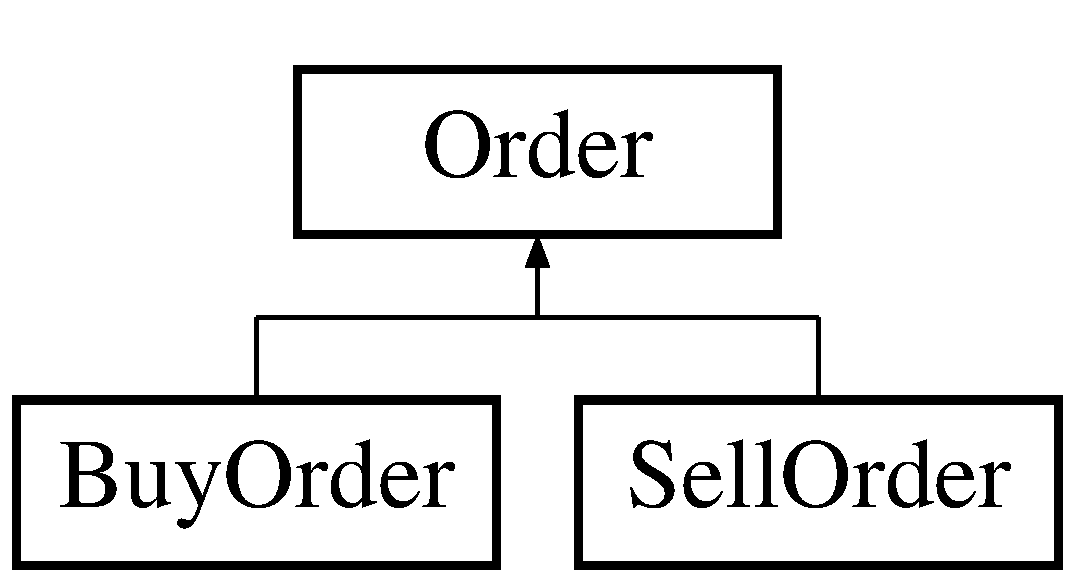
\includegraphics[height=2.000000cm]{class_order}
\end{center}
\end{figure}
\subsection*{Classes}
\begin{DoxyCompactItemize}
\item 
class \hyperlink{class_order_1_1_invalid_value}{Invalid\+Value}
\end{DoxyCompactItemize}
\subsection*{Public Member Functions}
\begin{DoxyCompactItemize}
\item 
\hyperlink{class_order_afd9bc0f1cf5ad376154ffde0e2727fbb}{Order} (ifstream \&in)
\item 
\hyperlink{class_order_afdda61d21957bffaf29e666ee6741bdc}{Order} (string s, double value, unsigned quant)
\item 
virtual \hyperlink{class_order_aa29be853510781d514722f857ab1698a}{$\sim$\+Order} ()=default
\item 
\hyperlink{class_date}{Date} \hyperlink{class_order_a8ffb9095f78f8a3b1942e7995516007c}{get\+Date\+Placed} () const
\item 
string \hyperlink{class_order_aa008956fd77ac3d254117443b7d916fa}{get\+Stock} () const
\item 
double \hyperlink{class_order_a7e93f84ff8b0468aef7e7ee23ea1979c}{get\+Value} () const
\item 
unsigned \hyperlink{class_order_a1d34436da1dbc3ffad588505eca5ff49}{get\+Quantity} () const
\item 
void \hyperlink{class_order_a718aea4e96286f2333222d6414eaa317}{print\+Info} () const
\item 
virtual nif\+\_\+t \hyperlink{class_order_a9831f386726f74ee20eea13a46282e13}{get\+Client\+N\+IF} () const =0
\item 
virtual \hyperlink{class_transaction}{Transaction} $\ast$ \hyperlink{class_order_a85d5de18c8664085619e3a5c74d47a25}{operator()} (\hyperlink{class_order}{Order} $\ast$o)=0
\item 
virtual void \hyperlink{class_order_a83989bde0a9b40cbeb0e87c965f6096e}{save\+Changes} (ofstream \&out) const
\end{DoxyCompactItemize}
\subsection*{Protected Attributes}
\begin{DoxyCompactItemize}
\item 
string \hyperlink{class_order_aafb6dfab2a1c253eefd78840b27dcd2e}{stock}
\item 
double \hyperlink{class_order_ab5d512fb35483413b9fe200d58324c2e}{value\+Per\+Stock}
\item 
unsigned \hyperlink{class_order_ab02e2baeb8c57217a20c9124df3ba11d}{quantity}
\item 
\hyperlink{class_date}{Date} \hyperlink{class_order_a23f58bb3f0162aac8c91a8a14136990c}{date\+Placed}
\end{DoxyCompactItemize}


\subsection{Detailed Description}
Abstract Base class used to represent an order. 

\subsection{Constructor \& Destructor Documentation}
\mbox{\Hypertarget{class_order_afd9bc0f1cf5ad376154ffde0e2727fbb}\label{class_order_afd9bc0f1cf5ad376154ffde0e2727fbb}} 
\index{Order@{Order}!Order@{Order}}
\index{Order@{Order}!Order@{Order}}
\subsubsection{\texorpdfstring{Order()}{Order()}\hspace{0.1cm}{\footnotesize\ttfamily [1/2]}}
{\footnotesize\ttfamily Order\+::\+Order (\begin{DoxyParamCaption}\item[{ifstream \&}]{in }\end{DoxyParamCaption})}

A constructor. The construtor creates an order object, reading the data from the input stream passed as argument. 
\begin{DoxyParams}{Parameters}
{\em in} & The input stream to read from in order to build the order object. \\
\hline
\end{DoxyParams}
\mbox{\Hypertarget{class_order_afdda61d21957bffaf29e666ee6741bdc}\label{class_order_afdda61d21957bffaf29e666ee6741bdc}} 
\index{Order@{Order}!Order@{Order}}
\index{Order@{Order}!Order@{Order}}
\subsubsection{\texorpdfstring{Order()}{Order()}\hspace{0.1cm}{\footnotesize\ttfamily [2/2]}}
{\footnotesize\ttfamily Order\+::\+Order (\begin{DoxyParamCaption}\item[{string}]{s,  }\item[{double}]{value,  }\item[{unsigned}]{quant }\end{DoxyParamCaption})}

A constructor. The construtor creates an order object using the data passed as arguments. 
\begin{DoxyParams}{Parameters}
{\em s} & A string with the stock name. \\
\hline
{\em value} & A double with the value per stock. \\
\hline
{\em quant} & An unsigned with the stock quantity. \\
\hline
\end{DoxyParams}
\mbox{\Hypertarget{class_order_aa29be853510781d514722f857ab1698a}\label{class_order_aa29be853510781d514722f857ab1698a}} 
\index{Order@{Order}!````~Order@{$\sim$\+Order}}
\index{````~Order@{$\sim$\+Order}!Order@{Order}}
\subsubsection{\texorpdfstring{$\sim$\+Order()}{~Order()}}
{\footnotesize\ttfamily virtual Order\+::$\sim$\+Order (\begin{DoxyParamCaption}{ }\end{DoxyParamCaption})\hspace{0.3cm}{\ttfamily [virtual]}, {\ttfamily [default]}}

A virtual destructor. 

\subsection{Member Function Documentation}
\mbox{\Hypertarget{class_order_a9831f386726f74ee20eea13a46282e13}\label{class_order_a9831f386726f74ee20eea13a46282e13}} 
\index{Order@{Order}!get\+Client\+N\+IF@{get\+Client\+N\+IF}}
\index{get\+Client\+N\+IF@{get\+Client\+N\+IF}!Order@{Order}}
\subsubsection{\texorpdfstring{get\+Client\+N\+I\+F()}{getClientNIF()}}
{\footnotesize\ttfamily virtual nif\+\_\+t Order\+::get\+Client\+N\+IF (\begin{DoxyParamCaption}{ }\end{DoxyParamCaption}) const\hspace{0.3cm}{\ttfamily [pure virtual]}}

A const abstract member function that returns the N\+IF of the client associated with the \hyperlink{class_order}{Order}. \begin{DoxyReturn}{Returns}
The N\+IF of the Buyer/\+Seller associated with the \hyperlink{class_order}{Order}. 
\end{DoxyReturn}


Implemented in \hyperlink{class_sell_order_a2f34e30d8bc5c891c40d8b80342cc34d}{Sell\+Order}, and \hyperlink{class_buy_order_ab79597b9bf0656216b2283bfa3a650e0}{Buy\+Order}.

\mbox{\Hypertarget{class_order_a8ffb9095f78f8a3b1942e7995516007c}\label{class_order_a8ffb9095f78f8a3b1942e7995516007c}} 
\index{Order@{Order}!get\+Date\+Placed@{get\+Date\+Placed}}
\index{get\+Date\+Placed@{get\+Date\+Placed}!Order@{Order}}
\subsubsection{\texorpdfstring{get\+Date\+Placed()}{getDatePlaced()}}
{\footnotesize\ttfamily \hyperlink{class_date}{Date} Order\+::get\+Date\+Placed (\begin{DoxyParamCaption}{ }\end{DoxyParamCaption}) const}

A const member function with no arguments to get the orders\textquotesingle{}s place date. \begin{DoxyReturn}{Returns}
A \hyperlink{class_date}{Date} object , the date when the order was placed. 
\end{DoxyReturn}
\mbox{\Hypertarget{class_order_a1d34436da1dbc3ffad588505eca5ff49}\label{class_order_a1d34436da1dbc3ffad588505eca5ff49}} 
\index{Order@{Order}!get\+Quantity@{get\+Quantity}}
\index{get\+Quantity@{get\+Quantity}!Order@{Order}}
\subsubsection{\texorpdfstring{get\+Quantity()}{getQuantity()}}
{\footnotesize\ttfamily unsigned Order\+::get\+Quantity (\begin{DoxyParamCaption}{ }\end{DoxyParamCaption}) const}

A const member function with no arguments to get the order stock quantity. \begin{DoxyReturn}{Returns}
An unsigned, the quantity of stock. 
\end{DoxyReturn}
\mbox{\Hypertarget{class_order_aa008956fd77ac3d254117443b7d916fa}\label{class_order_aa008956fd77ac3d254117443b7d916fa}} 
\index{Order@{Order}!get\+Stock@{get\+Stock}}
\index{get\+Stock@{get\+Stock}!Order@{Order}}
\subsubsection{\texorpdfstring{get\+Stock()}{getStock()}}
{\footnotesize\ttfamily string Order\+::get\+Stock (\begin{DoxyParamCaption}{ }\end{DoxyParamCaption}) const}

A const member function with no arguments to get the orders\textquotesingle{}s stock name. \begin{DoxyReturn}{Returns}
A string that is the name of the stock. 
\end{DoxyReturn}
\mbox{\Hypertarget{class_order_a7e93f84ff8b0468aef7e7ee23ea1979c}\label{class_order_a7e93f84ff8b0468aef7e7ee23ea1979c}} 
\index{Order@{Order}!get\+Value@{get\+Value}}
\index{get\+Value@{get\+Value}!Order@{Order}}
\subsubsection{\texorpdfstring{get\+Value()}{getValue()}}
{\footnotesize\ttfamily double Order\+::get\+Value (\begin{DoxyParamCaption}{ }\end{DoxyParamCaption}) const}

A const member function with no arguments to get the value per stock. \begin{DoxyReturn}{Returns}
A double, the value per stock. 
\end{DoxyReturn}
\mbox{\Hypertarget{class_order_a85d5de18c8664085619e3a5c74d47a25}\label{class_order_a85d5de18c8664085619e3a5c74d47a25}} 
\index{Order@{Order}!operator()@{operator()}}
\index{operator()@{operator()}!Order@{Order}}
\subsubsection{\texorpdfstring{operator()()}{operator()()}}
{\footnotesize\ttfamily virtual \hyperlink{class_transaction}{Transaction}$\ast$ Order\+::operator() (\begin{DoxyParamCaption}\item[{\hyperlink{class_order}{Order} $\ast$}]{o }\end{DoxyParamCaption})\hspace{0.3cm}{\ttfamily [pure virtual]}}

Abstract overload of function operator. Cheks whether this instance of an \hyperlink{class_order}{Order} Object can be fulfilled by the provided \hyperlink{class_order}{Order}. 
\begin{DoxyParams}{Parameters}
{\em an} & \hyperlink{class_order}{Order} pointer \\
\hline
\end{DoxyParams}
\begin{DoxyReturn}{Returns}
A pointer to the transaction generated if successful, N\+U\+LL otherwise. 
\end{DoxyReturn}


Implemented in \hyperlink{class_sell_order_ae4e19807431bcd87c7126d0c644ff209}{Sell\+Order}, and \hyperlink{class_buy_order_a45641eed13ea191fff675745a618b9f5}{Buy\+Order}.

\mbox{\Hypertarget{class_order_a718aea4e96286f2333222d6414eaa317}\label{class_order_a718aea4e96286f2333222d6414eaa317}} 
\index{Order@{Order}!print\+Info@{print\+Info}}
\index{print\+Info@{print\+Info}!Order@{Order}}
\subsubsection{\texorpdfstring{print\+Info()}{printInfo()}}
{\footnotesize\ttfamily void Order\+::print\+Info (\begin{DoxyParamCaption}{ }\end{DoxyParamCaption}) const}

A const member function that prints the order information. \mbox{\Hypertarget{class_order_a83989bde0a9b40cbeb0e87c965f6096e}\label{class_order_a83989bde0a9b40cbeb0e87c965f6096e}} 
\index{Order@{Order}!save\+Changes@{save\+Changes}}
\index{save\+Changes@{save\+Changes}!Order@{Order}}
\subsubsection{\texorpdfstring{save\+Changes()}{saveChanges()}}
{\footnotesize\ttfamily void Order\+::save\+Changes (\begin{DoxyParamCaption}\item[{ofstream \&}]{out }\end{DoxyParamCaption}) const\hspace{0.3cm}{\ttfamily [virtual]}}

A virtual function to save changes in the derived classes. 

Reimplemented in \hyperlink{class_sell_order_a81c6ea39652c38a718803c036767787f}{Sell\+Order}, and \hyperlink{class_buy_order_aa4f087d0dbc1f6e8937c0b3679fc2f7b}{Buy\+Order}.



\subsection{Member Data Documentation}
\mbox{\Hypertarget{class_order_a23f58bb3f0162aac8c91a8a14136990c}\label{class_order_a23f58bb3f0162aac8c91a8a14136990c}} 
\index{Order@{Order}!date\+Placed@{date\+Placed}}
\index{date\+Placed@{date\+Placed}!Order@{Order}}
\subsubsection{\texorpdfstring{date\+Placed}{datePlaced}}
{\footnotesize\ttfamily \hyperlink{class_date}{Date} Order\+::date\+Placed\hspace{0.3cm}{\ttfamily [protected]}}

\hyperlink{class_date}{Date} date\+Placed. The date when the order was placed. \mbox{\Hypertarget{class_order_ab02e2baeb8c57217a20c9124df3ba11d}\label{class_order_ab02e2baeb8c57217a20c9124df3ba11d}} 
\index{Order@{Order}!quantity@{quantity}}
\index{quantity@{quantity}!Order@{Order}}
\subsubsection{\texorpdfstring{quantity}{quantity}}
{\footnotesize\ttfamily unsigned Order\+::quantity\hspace{0.3cm}{\ttfamily [protected]}}

unsigned quantity. An unsigned with the stock quantity. \mbox{\Hypertarget{class_order_aafb6dfab2a1c253eefd78840b27dcd2e}\label{class_order_aafb6dfab2a1c253eefd78840b27dcd2e}} 
\index{Order@{Order}!stock@{stock}}
\index{stock@{stock}!Order@{Order}}
\subsubsection{\texorpdfstring{stock}{stock}}
{\footnotesize\ttfamily string Order\+::stock\hspace{0.3cm}{\ttfamily [protected]}}

string stock. A string with stock name. \mbox{\Hypertarget{class_order_ab5d512fb35483413b9fe200d58324c2e}\label{class_order_ab5d512fb35483413b9fe200d58324c2e}} 
\index{Order@{Order}!value\+Per\+Stock@{value\+Per\+Stock}}
\index{value\+Per\+Stock@{value\+Per\+Stock}!Order@{Order}}
\subsubsection{\texorpdfstring{value\+Per\+Stock}{valuePerStock}}
{\footnotesize\ttfamily double Order\+::value\+Per\+Stock\hspace{0.3cm}{\ttfamily [protected]}}

value\+Per\+Stock. A double with the stock value. 

The documentation for this class was generated from the following files\+:\begin{DoxyCompactItemize}
\item 
D\+:/\+Projetos\+C++/\+A\+E\+D\+Av2/\+Stock\+Market/Order.\+h\item 
D\+:/\+Projetos\+C++/\+A\+E\+D\+Av2/\+Stock\+Market/Order.\+cpp\end{DoxyCompactItemize}

\hypertarget{class_sell_order}{}\section{Sell\+Order Class Reference}
\label{class_sell_order}\index{Sell\+Order@{Sell\+Order}}


{\ttfamily \#include $<$Order.\+h$>$}

Inheritance diagram for Sell\+Order\+:\begin{figure}[H]
\begin{center}
\leavevmode
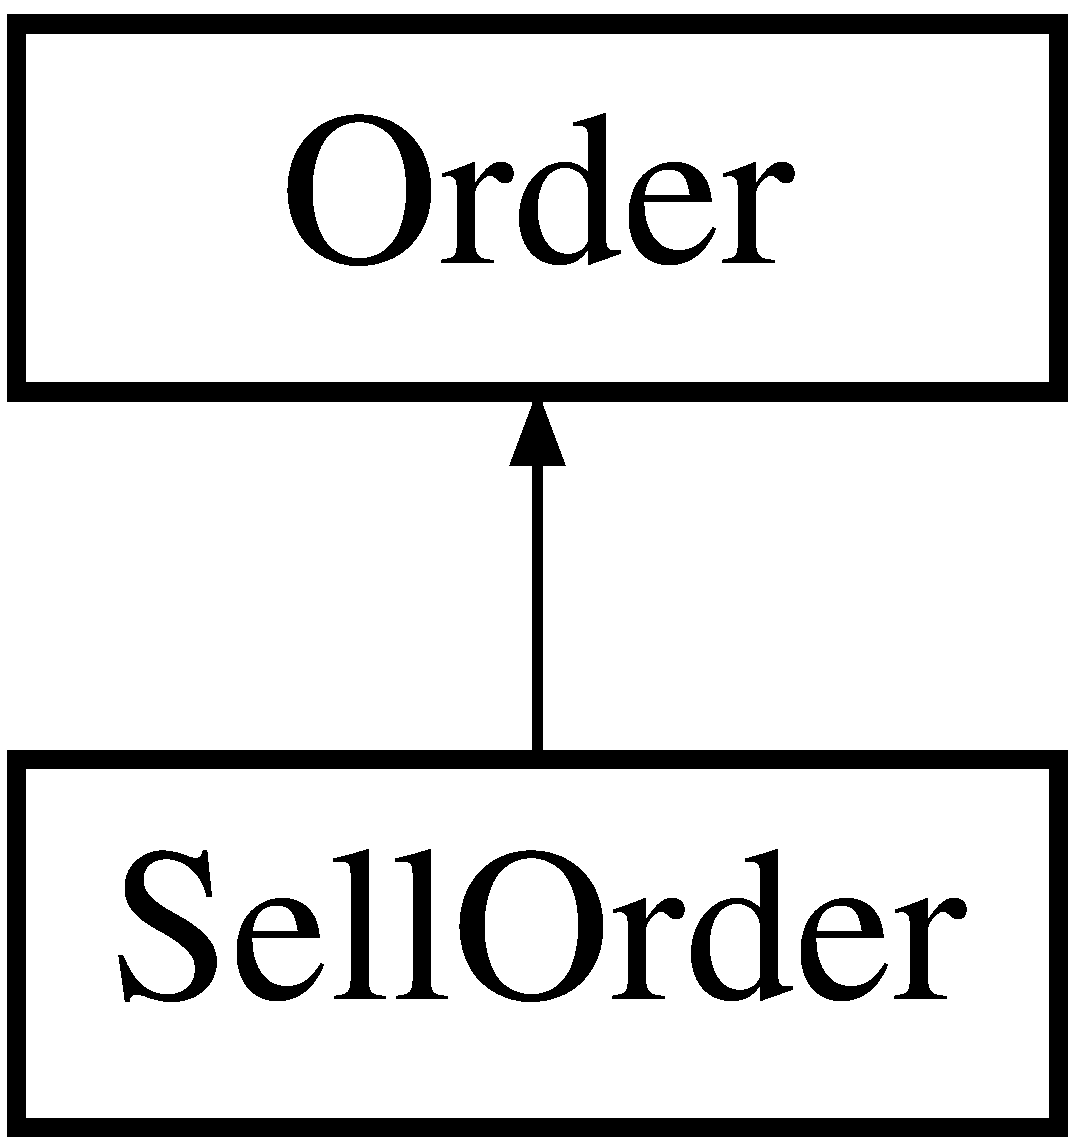
\includegraphics[height=2.000000cm]{class_sell_order}
\end{center}
\end{figure}
\subsection*{Public Member Functions}
\begin{DoxyCompactItemize}
\item 
\hyperlink{class_sell_order_ac89fdde112f2f9aac52633a2d9507bea}{Sell\+Order} (ifstream \&in)
\begin{DoxyCompactList}\small\item\em /// \end{DoxyCompactList}\item 
\hyperlink{class_sell_order_a19145616a9cceec182bdcb00816b89c5}{Sell\+Order} (string \hyperlink{class_order_aafb6dfab2a1c253eefd78840b27dcd2e}{stock}, double val, unsigned \hyperlink{class_order_ab02e2baeb8c57217a20c9124df3ba11d}{quantity}, nif\+\_\+t \hyperlink{class_sell_order_a986130b91a0dc2f234dffc10b24c3183}{seller\+N\+IF})
\item 
nif\+\_\+t \hyperlink{class_sell_order_a2f34e30d8bc5c891c40d8b80342cc34d}{get\+Client\+N\+IF} () const
\item 
\hyperlink{class_transaction}{Transaction} $\ast$ \hyperlink{class_sell_order_ae4e19807431bcd87c7126d0c644ff209}{operator()} (\hyperlink{class_order}{Order} $\ast$o)
\item 
void \hyperlink{class_sell_order_a81c6ea39652c38a718803c036767787f}{save\+Changes} (ofstream \&out) const
\end{DoxyCompactItemize}
\subsection*{Private Attributes}
\begin{DoxyCompactItemize}
\item 
\mbox{\Hypertarget{class_sell_order_a9c9a7419b6974313ef6b5e4e16be6b8a}\label{class_sell_order_a9c9a7419b6974313ef6b5e4e16be6b8a}} 
friend {\bfseries Buy\+Order}
\item 
nif\+\_\+t \hyperlink{class_sell_order_a986130b91a0dc2f234dffc10b24c3183}{seller\+N\+IF}
\end{DoxyCompactItemize}
\subsection*{Additional Inherited Members}


\subsection{Detailed Description}
Class used to represent a sell order. Derives from \hyperlink{class_order}{Order}. 

\subsection{Constructor \& Destructor Documentation}
\mbox{\Hypertarget{class_sell_order_ac89fdde112f2f9aac52633a2d9507bea}\label{class_sell_order_ac89fdde112f2f9aac52633a2d9507bea}} 
\index{Sell\+Order@{Sell\+Order}!Sell\+Order@{Sell\+Order}}
\index{Sell\+Order@{Sell\+Order}!Sell\+Order@{Sell\+Order}}
\subsubsection{\texorpdfstring{Sell\+Order()}{SellOrder()}\hspace{0.1cm}{\footnotesize\ttfamily [1/2]}}
{\footnotesize\ttfamily Sell\+Order\+::\+Sell\+Order (\begin{DoxyParamCaption}\item[{ifstream \&}]{in }\end{DoxyParamCaption})}



/// 

A constructor. The construtor creates a \hyperlink{class_sell_order}{Sell\+Order} object, reading the data from the input stream passed as argument. 
\begin{DoxyParams}{Parameters}
{\em in} & The input stream to read from in order to build the \hyperlink{class_sell_order}{Sell\+Order} object. \\
\hline
\end{DoxyParams}
\mbox{\Hypertarget{class_sell_order_a19145616a9cceec182bdcb00816b89c5}\label{class_sell_order_a19145616a9cceec182bdcb00816b89c5}} 
\index{Sell\+Order@{Sell\+Order}!Sell\+Order@{Sell\+Order}}
\index{Sell\+Order@{Sell\+Order}!Sell\+Order@{Sell\+Order}}
\subsubsection{\texorpdfstring{Sell\+Order()}{SellOrder()}\hspace{0.1cm}{\footnotesize\ttfamily [2/2]}}
{\footnotesize\ttfamily Sell\+Order\+::\+Sell\+Order (\begin{DoxyParamCaption}\item[{string}]{stock,  }\item[{double}]{val,  }\item[{unsigned}]{quantity,  }\item[{nif\+\_\+t}]{seller\+N\+IF }\end{DoxyParamCaption})}

A constructor. The construtor creates a \hyperlink{class_sell_order}{Sell\+Order} object using the data passed as arguments. 
\begin{DoxyParams}{Parameters}
{\em stock} & A string with the stock name. \\
\hline
{\em val} & A double with the value per stock. \\
\hline
{\em quantity} & An unsigned with the stock quantity. \\
\hline
{\em seller\+N\+IF} & The seller\textquotesingle{}s N\+IF. \\
\hline
\end{DoxyParams}


\subsection{Member Function Documentation}
\mbox{\Hypertarget{class_sell_order_a2f34e30d8bc5c891c40d8b80342cc34d}\label{class_sell_order_a2f34e30d8bc5c891c40d8b80342cc34d}} 
\index{Sell\+Order@{Sell\+Order}!get\+Client\+N\+IF@{get\+Client\+N\+IF}}
\index{get\+Client\+N\+IF@{get\+Client\+N\+IF}!Sell\+Order@{Sell\+Order}}
\subsubsection{\texorpdfstring{get\+Client\+N\+I\+F()}{getClientNIF()}}
{\footnotesize\ttfamily nif\+\_\+t Sell\+Order\+::get\+Client\+N\+IF (\begin{DoxyParamCaption}{ }\end{DoxyParamCaption}) const\hspace{0.3cm}{\ttfamily [virtual]}}

A const member function that returns the N\+IF of the client associated with this \hyperlink{class_sell_order}{Sell\+Order}. \begin{DoxyReturn}{Returns}
The N\+IF of the Seller associated with this \hyperlink{class_order}{Order}. 
\end{DoxyReturn}


Implements \hyperlink{class_order_a9831f386726f74ee20eea13a46282e13}{Order}.

\mbox{\Hypertarget{class_sell_order_ae4e19807431bcd87c7126d0c644ff209}\label{class_sell_order_ae4e19807431bcd87c7126d0c644ff209}} 
\index{Sell\+Order@{Sell\+Order}!operator()@{operator()}}
\index{operator()@{operator()}!Sell\+Order@{Sell\+Order}}
\subsubsection{\texorpdfstring{operator()()}{operator()()}}
{\footnotesize\ttfamily \hyperlink{class_transaction}{Transaction} $\ast$ Sell\+Order\+::operator() (\begin{DoxyParamCaption}\item[{\hyperlink{class_order}{Order} $\ast$}]{o }\end{DoxyParamCaption})\hspace{0.3cm}{\ttfamily [virtual]}}

Overload of operator() for class \hyperlink{class_order}{Order}. 
\begin{DoxyParams}{Parameters}
{\em o} & Pointer of an object \hyperlink{class_order}{Order}. \\
\hline
\end{DoxyParams}
\begin{DoxyReturn}{Returns}
A transaction type object. 
\end{DoxyReturn}


Implements \hyperlink{class_order_a85d5de18c8664085619e3a5c74d47a25}{Order}.

\mbox{\Hypertarget{class_sell_order_a81c6ea39652c38a718803c036767787f}\label{class_sell_order_a81c6ea39652c38a718803c036767787f}} 
\index{Sell\+Order@{Sell\+Order}!save\+Changes@{save\+Changes}}
\index{save\+Changes@{save\+Changes}!Sell\+Order@{Sell\+Order}}
\subsubsection{\texorpdfstring{save\+Changes()}{saveChanges()}}
{\footnotesize\ttfamily void Sell\+Order\+::save\+Changes (\begin{DoxyParamCaption}\item[{ofstream \&}]{out }\end{DoxyParamCaption}) const\hspace{0.3cm}{\ttfamily [virtual]}}

A const memeber function to save changes in an output stream. 
\begin{DoxyParams}{Parameters}
{\em out} & The outstream file to write to. \\
\hline
\end{DoxyParams}


Reimplemented from \hyperlink{class_order_a83989bde0a9b40cbeb0e87c965f6096e}{Order}.



\subsection{Member Data Documentation}
\mbox{\Hypertarget{class_sell_order_a986130b91a0dc2f234dffc10b24c3183}\label{class_sell_order_a986130b91a0dc2f234dffc10b24c3183}} 
\index{Sell\+Order@{Sell\+Order}!seller\+N\+IF@{seller\+N\+IF}}
\index{seller\+N\+IF@{seller\+N\+IF}!Sell\+Order@{Sell\+Order}}
\subsubsection{\texorpdfstring{seller\+N\+IF}{sellerNIF}}
{\footnotesize\ttfamily nif\+\_\+t Sell\+Order\+::seller\+N\+IF\hspace{0.3cm}{\ttfamily [private]}}

nif\+\_\+t seller\+N\+IF. The N\+IF of the seller associated with this \hyperlink{class_order}{Order}. 

The documentation for this class was generated from the following files\+:\begin{DoxyCompactItemize}
\item 
D\+:/\+Projetos\+C++/\+A\+E\+D\+Av2/\+Stock\+Market/Order.\+h\item 
D\+:/\+Projetos\+C++/\+A\+E\+D\+Av2/\+Stock\+Market/Order.\+cpp\end{DoxyCompactItemize}

\hypertarget{class_transaction}{}\section{Transaction Class Reference}
\label{class_transaction}\index{Transaction@{Transaction}}


{\ttfamily \#include $<$Transaction.\+h$>$}

\subsection*{Public Member Functions}
\begin{DoxyCompactItemize}
\item 
\hyperlink{class_transaction_a0c8031bed6e7a45eda7bc2ca8f40e851}{Transaction} ()=default
\item 
\hyperlink{class_transaction_a2bbb78694a94a630cb1e9e741dc120a7}{Transaction} (ifstream \&in)
\item 
\hyperlink{class_transaction_abd1826b5a0499ddac290a4f1297e7455}{Transaction} (nif\+\_\+t \hyperlink{class_transaction_a3db24320f561ae3a72887e7a34b19917}{buyer\+N\+IF}, nif\+\_\+t \hyperlink{class_transaction_a4f779b188a508987aa610e4274765059}{seller\+N\+IF}, string \hyperlink{class_transaction_ae0fd78bf4db4a8dc6d4d931f107a6213}{stock}, double \hyperlink{class_transaction_a75d644553218251b030313776ff33f51}{value}, unsigned \hyperlink{class_transaction_a32045bcdce9ba390cf1c646578e29fd3}{quantity})
\item 
string \hyperlink{class_transaction_af6582ddc59e9cfa99a7ef178216799be}{get\+Stock} () const
\item 
double \hyperlink{class_transaction_a95976b2e60b66d766edf4db534324db4}{get\+Value} () const
\item 
unsigned \hyperlink{class_transaction_ab3bfaa0469e1f45c5bd5dc164ac3c850}{get\+Quantity} () const
\item 
nif\+\_\+t \hyperlink{class_transaction_a3c3a57a3240bece392c56ff41bc3c21b}{get\+Seller\+N\+IF} () const
\item 
nif\+\_\+t \hyperlink{class_transaction_afa91c88bb936d8bd8480ac36b599649b}{get\+Buyer\+N\+IF} () const
\item 
\hyperlink{class_date}{Date} \hyperlink{class_transaction_af2ef4a1ef82f9ff5d34dae7234211589}{get\+Date} () const
\item 
void \hyperlink{class_transaction_a3c0c3c4a64c5b3d20c420708357a86be}{save\+Changes} (ofstream \&out) const
\end{DoxyCompactItemize}
\subsection*{Private Attributes}
\begin{DoxyCompactItemize}
\item 
nif\+\_\+t \hyperlink{class_transaction_a4f779b188a508987aa610e4274765059}{seller\+N\+IF}
\item 
nif\+\_\+t \hyperlink{class_transaction_a3db24320f561ae3a72887e7a34b19917}{buyer\+N\+IF}
\item 
string \hyperlink{class_transaction_ae0fd78bf4db4a8dc6d4d931f107a6213}{stock}
\item 
double \hyperlink{class_transaction_a75d644553218251b030313776ff33f51}{value}
\item 
unsigned \hyperlink{class_transaction_a32045bcdce9ba390cf1c646578e29fd3}{quantity}
\item 
\hyperlink{class_date}{Date} \hyperlink{class_transaction_a94ff0c865db09881fa3becfdad25ce5d}{time\+\_\+stamp}
\end{DoxyCompactItemize}
\subsection*{Friends}
\begin{DoxyCompactItemize}
\item 
ostream \& \hyperlink{class_transaction_a8d6d6be74010b57302f4567e06cdbed3}{operator$<$$<$} (ostream \&, const \hyperlink{class_transaction}{Transaction} \&)
\end{DoxyCompactItemize}


\subsection{Detailed Description}
A class used to represent a transaction. 

\subsection{Constructor \& Destructor Documentation}
\mbox{\Hypertarget{class_transaction_a0c8031bed6e7a45eda7bc2ca8f40e851}\label{class_transaction_a0c8031bed6e7a45eda7bc2ca8f40e851}} 
\index{Transaction@{Transaction}!Transaction@{Transaction}}
\index{Transaction@{Transaction}!Transaction@{Transaction}}
\subsubsection{\texorpdfstring{Transaction()}{Transaction()}\hspace{0.1cm}{\footnotesize\ttfamily [1/3]}}
{\footnotesize\ttfamily Transaction\+::\+Transaction (\begin{DoxyParamCaption}{ }\end{DoxyParamCaption})\hspace{0.3cm}{\ttfamily [default]}}

A default constructor. \mbox{\Hypertarget{class_transaction_a2bbb78694a94a630cb1e9e741dc120a7}\label{class_transaction_a2bbb78694a94a630cb1e9e741dc120a7}} 
\index{Transaction@{Transaction}!Transaction@{Transaction}}
\index{Transaction@{Transaction}!Transaction@{Transaction}}
\subsubsection{\texorpdfstring{Transaction()}{Transaction()}\hspace{0.1cm}{\footnotesize\ttfamily [2/3]}}
{\footnotesize\ttfamily Transaction\+::\+Transaction (\begin{DoxyParamCaption}\item[{ifstream \&}]{in }\end{DoxyParamCaption})}

A constructor. The construtor creates a transaction object, reading the data from the input stream passed as argument. 
\begin{DoxyParams}{Parameters}
{\em in} & The input stream to read from in order to build the transaction object. \\
\hline
\end{DoxyParams}
\mbox{\Hypertarget{class_transaction_abd1826b5a0499ddac290a4f1297e7455}\label{class_transaction_abd1826b5a0499ddac290a4f1297e7455}} 
\index{Transaction@{Transaction}!Transaction@{Transaction}}
\index{Transaction@{Transaction}!Transaction@{Transaction}}
\subsubsection{\texorpdfstring{Transaction()}{Transaction()}\hspace{0.1cm}{\footnotesize\ttfamily [3/3]}}
{\footnotesize\ttfamily Transaction\+::\+Transaction (\begin{DoxyParamCaption}\item[{nif\+\_\+t}]{buyer\+N\+IF,  }\item[{nif\+\_\+t}]{seller\+N\+IF,  }\item[{string}]{stock,  }\item[{double}]{value,  }\item[{unsigned}]{quantity }\end{DoxyParamCaption})}

A constructor. The construtor creates a transaction object using the data passed as arguments. 
\begin{DoxyParams}{Parameters}
{\em buyer\+N\+IF} & The N\+IF from the buyer. \\
\hline
{\em seller\+N\+IF} & The N\+IF from the seller. \\
\hline
{\em stock} & The stock name. \\
\hline
{\em value} & The value of the stock. \\
\hline
{\em quantity} & The amount of stock. \\
\hline
\end{DoxyParams}


\subsection{Member Function Documentation}
\mbox{\Hypertarget{class_transaction_afa91c88bb936d8bd8480ac36b599649b}\label{class_transaction_afa91c88bb936d8bd8480ac36b599649b}} 
\index{Transaction@{Transaction}!get\+Buyer\+N\+IF@{get\+Buyer\+N\+IF}}
\index{get\+Buyer\+N\+IF@{get\+Buyer\+N\+IF}!Transaction@{Transaction}}
\subsubsection{\texorpdfstring{get\+Buyer\+N\+I\+F()}{getBuyerNIF()}}
{\footnotesize\ttfamily nif\+\_\+t Transaction\+::get\+Buyer\+N\+IF (\begin{DoxyParamCaption}{ }\end{DoxyParamCaption}) const}

A const member function with no arguments to get the transaction\textquotesingle{}s buyer N\+IF. \begin{DoxyReturn}{Returns}
A nif\+\_\+t , the buyer N\+IF. 
\end{DoxyReturn}
\mbox{\Hypertarget{class_transaction_af2ef4a1ef82f9ff5d34dae7234211589}\label{class_transaction_af2ef4a1ef82f9ff5d34dae7234211589}} 
\index{Transaction@{Transaction}!get\+Date@{get\+Date}}
\index{get\+Date@{get\+Date}!Transaction@{Transaction}}
\subsubsection{\texorpdfstring{get\+Date()}{getDate()}}
{\footnotesize\ttfamily \hyperlink{class_date}{Date} Transaction\+::get\+Date (\begin{DoxyParamCaption}{ }\end{DoxyParamCaption}) const}

A const member function with no arguments to get the transaction\textquotesingle{}s date. \begin{DoxyReturn}{Returns}
A \hyperlink{class_date}{Date} object , the date of the transaction. 
\end{DoxyReturn}
\mbox{\Hypertarget{class_transaction_ab3bfaa0469e1f45c5bd5dc164ac3c850}\label{class_transaction_ab3bfaa0469e1f45c5bd5dc164ac3c850}} 
\index{Transaction@{Transaction}!get\+Quantity@{get\+Quantity}}
\index{get\+Quantity@{get\+Quantity}!Transaction@{Transaction}}
\subsubsection{\texorpdfstring{get\+Quantity()}{getQuantity()}}
{\footnotesize\ttfamily unsigned Transaction\+::get\+Quantity (\begin{DoxyParamCaption}{ }\end{DoxyParamCaption}) const}

A const member function with no arguments to get the transaction\textquotesingle{}s quantity of stock. \begin{DoxyReturn}{Returns}
An unsigned, the quantity. 
\end{DoxyReturn}
\mbox{\Hypertarget{class_transaction_a3c3a57a3240bece392c56ff41bc3c21b}\label{class_transaction_a3c3a57a3240bece392c56ff41bc3c21b}} 
\index{Transaction@{Transaction}!get\+Seller\+N\+IF@{get\+Seller\+N\+IF}}
\index{get\+Seller\+N\+IF@{get\+Seller\+N\+IF}!Transaction@{Transaction}}
\subsubsection{\texorpdfstring{get\+Seller\+N\+I\+F()}{getSellerNIF()}}
{\footnotesize\ttfamily nif\+\_\+t Transaction\+::get\+Seller\+N\+IF (\begin{DoxyParamCaption}{ }\end{DoxyParamCaption}) const}

A const member function with no arguments to get the transaction\textquotesingle{}s seller N\+IF. \begin{DoxyReturn}{Returns}
A nif\+\_\+t , the seller N\+IF. 
\end{DoxyReturn}
\mbox{\Hypertarget{class_transaction_af6582ddc59e9cfa99a7ef178216799be}\label{class_transaction_af6582ddc59e9cfa99a7ef178216799be}} 
\index{Transaction@{Transaction}!get\+Stock@{get\+Stock}}
\index{get\+Stock@{get\+Stock}!Transaction@{Transaction}}
\subsubsection{\texorpdfstring{get\+Stock()}{getStock()}}
{\footnotesize\ttfamily string Transaction\+::get\+Stock (\begin{DoxyParamCaption}{ }\end{DoxyParamCaption}) const}

A const member function with no arguments to get the transaction\textquotesingle{}s Stock name. \begin{DoxyReturn}{Returns}
A string, the Stock\textquotesingle{}s name. 
\end{DoxyReturn}
\mbox{\Hypertarget{class_transaction_a95976b2e60b66d766edf4db534324db4}\label{class_transaction_a95976b2e60b66d766edf4db534324db4}} 
\index{Transaction@{Transaction}!get\+Value@{get\+Value}}
\index{get\+Value@{get\+Value}!Transaction@{Transaction}}
\subsubsection{\texorpdfstring{get\+Value()}{getValue()}}
{\footnotesize\ttfamily double Transaction\+::get\+Value (\begin{DoxyParamCaption}{ }\end{DoxyParamCaption}) const}

A const member function with no arguments to get the transaction\textquotesingle{}s Value Per Stock. \begin{DoxyReturn}{Returns}
A double, the value per stock transactioned. 
\end{DoxyReturn}
\mbox{\Hypertarget{class_transaction_a3c0c3c4a64c5b3d20c420708357a86be}\label{class_transaction_a3c0c3c4a64c5b3d20c420708357a86be}} 
\index{Transaction@{Transaction}!save\+Changes@{save\+Changes}}
\index{save\+Changes@{save\+Changes}!Transaction@{Transaction}}
\subsubsection{\texorpdfstring{save\+Changes()}{saveChanges()}}
{\footnotesize\ttfamily void Transaction\+::save\+Changes (\begin{DoxyParamCaption}\item[{ofstream \&}]{out }\end{DoxyParamCaption}) const}

A const member function to write the transaction to a save file. 
\begin{DoxyParams}{Parameters}
{\em out} & The outputstream file to write to. \\
\hline
\end{DoxyParams}


\subsection{Friends And Related Function Documentation}
\mbox{\Hypertarget{class_transaction_a8d6d6be74010b57302f4567e06cdbed3}\label{class_transaction_a8d6d6be74010b57302f4567e06cdbed3}} 
\index{Transaction@{Transaction}!operator$<$$<$@{operator$<$$<$}}
\index{operator$<$$<$@{operator$<$$<$}!Transaction@{Transaction}}
\subsubsection{\texorpdfstring{operator$<$$<$}{operator<<}}
{\footnotesize\ttfamily ostream\& operator$<$$<$ (\begin{DoxyParamCaption}\item[{ostream \&}]{,  }\item[{const \hyperlink{class_transaction}{Transaction} \&}]{ }\end{DoxyParamCaption})\hspace{0.3cm}{\ttfamily [friend]}}

Overload of Operator $<$$<$ for class \hyperlink{class_transaction}{Transaction}. Prints the transaction in a human friendly way. 
\begin{DoxyParams}{Parameters}
{\em out} & The outstream to write to. \\
\hline
{\em t} & The transaction to be written. \\
\hline
\end{DoxyParams}
\begin{DoxyReturn}{Returns}
Returns the output stream to allow chainning 
\end{DoxyReturn}


\subsection{Member Data Documentation}
\mbox{\Hypertarget{class_transaction_a3db24320f561ae3a72887e7a34b19917}\label{class_transaction_a3db24320f561ae3a72887e7a34b19917}} 
\index{Transaction@{Transaction}!buyer\+N\+IF@{buyer\+N\+IF}}
\index{buyer\+N\+IF@{buyer\+N\+IF}!Transaction@{Transaction}}
\subsubsection{\texorpdfstring{buyer\+N\+IF}{buyerNIF}}
{\footnotesize\ttfamily nif\+\_\+t Transaction\+::buyer\+N\+IF\hspace{0.3cm}{\ttfamily [private]}}

nif\+\_\+t buyer\+N\+IF. The N\+IF from the client that bought the stock. \mbox{\Hypertarget{class_transaction_a32045bcdce9ba390cf1c646578e29fd3}\label{class_transaction_a32045bcdce9ba390cf1c646578e29fd3}} 
\index{Transaction@{Transaction}!quantity@{quantity}}
\index{quantity@{quantity}!Transaction@{Transaction}}
\subsubsection{\texorpdfstring{quantity}{quantity}}
{\footnotesize\ttfamily unsigned Transaction\+::quantity\hspace{0.3cm}{\ttfamily [private]}}

unsigned quantity. The quantity of stock. \mbox{\Hypertarget{class_transaction_a4f779b188a508987aa610e4274765059}\label{class_transaction_a4f779b188a508987aa610e4274765059}} 
\index{Transaction@{Transaction}!seller\+N\+IF@{seller\+N\+IF}}
\index{seller\+N\+IF@{seller\+N\+IF}!Transaction@{Transaction}}
\subsubsection{\texorpdfstring{seller\+N\+IF}{sellerNIF}}
{\footnotesize\ttfamily nif\+\_\+t Transaction\+::seller\+N\+IF\hspace{0.3cm}{\ttfamily [private]}}

nif\+\_\+t seller\+N\+IF. The N\+IF from the client that sold the stock. \mbox{\Hypertarget{class_transaction_ae0fd78bf4db4a8dc6d4d931f107a6213}\label{class_transaction_ae0fd78bf4db4a8dc6d4d931f107a6213}} 
\index{Transaction@{Transaction}!stock@{stock}}
\index{stock@{stock}!Transaction@{Transaction}}
\subsubsection{\texorpdfstring{stock}{stock}}
{\footnotesize\ttfamily string Transaction\+::stock\hspace{0.3cm}{\ttfamily [private]}}

string stock. The name of the stock product. \mbox{\Hypertarget{class_transaction_a94ff0c865db09881fa3becfdad25ce5d}\label{class_transaction_a94ff0c865db09881fa3becfdad25ce5d}} 
\index{Transaction@{Transaction}!time\+\_\+stamp@{time\+\_\+stamp}}
\index{time\+\_\+stamp@{time\+\_\+stamp}!Transaction@{Transaction}}
\subsubsection{\texorpdfstring{time\+\_\+stamp}{time\_stamp}}
{\footnotesize\ttfamily \hyperlink{class_date}{Date} Transaction\+::time\+\_\+stamp\hspace{0.3cm}{\ttfamily [private]}}

\hyperlink{class_date}{Date} time\+\_\+stamp. The time where the transaction occured. \mbox{\Hypertarget{class_transaction_a75d644553218251b030313776ff33f51}\label{class_transaction_a75d644553218251b030313776ff33f51}} 
\index{Transaction@{Transaction}!value@{value}}
\index{value@{value}!Transaction@{Transaction}}
\subsubsection{\texorpdfstring{value}{value}}
{\footnotesize\ttfamily double Transaction\+::value\hspace{0.3cm}{\ttfamily [private]}}

double value. The value of the stock. 

The documentation for this class was generated from the following files\+:\begin{DoxyCompactItemize}
\item 
D\+:/\+Projetos\+C++/\+A\+E\+D\+Av2/\+Stock\+Market/Transaction.\+h\item 
D\+:/\+Projetos\+C++/\+A\+E\+D\+Av2/\+Stock\+Market/Transaction.\+cpp\end{DoxyCompactItemize}

%--- End generated contents ---

% Index
\backmatter
\newpage
\phantomsection
\clearemptydoublepage
\addcontentsline{toc}{chapter}{Index}
\printindex

\end{document}
